\title{EE5311 -- Assignment 1}
\author{Joyen Benitto}
\date{\today}
\maketitle

\section{Problem 1}

\subsection*{Device Parameters}

The following long-channel/velocity-saturation parameters (sky130, 1.8 V process) are used throughout this problem:

\begin{itemize}
  \item nMOS: $V_{Tn} = 0.7$ V, $\mu_n = 0.025\ \text{m}^2/\text{Vs}$, $C_{oxn} = 8.34\ \text{fF}/\mu\text{m}^2$, $v_{satn} = 8\times10^4$ m/s, $\lambda_n = 0.2/\text{V}$
  \item pMOS: $|V_{Tp}| = 0.7$ V, $\mu_p = 0.009\ \text{m}^2/\text{Vs}$, $C_{oxp} = 8.16\ \text{fF}/\mu\text{m}^2$, $v_{satp} = 3\times10^4$ m/s, $\lambda_p = 0.2/\text{V}$
\end{itemize}

\subsection{Part (a): nMOS Transfer Characteristics}

Consider an nMOS transistor with $L = 0.15\ \mu\text{m}$ and $W = 0.42\ \mu\text{m}$, connected in a diode-connected configuration: the gate and drain are tied together to a swept input source $V_{in}$, the source and body are grounded, and the drain current $I_{ds}$ flows from $V_{in}$ into the drain.

\begin{enumerate}
  \item Determine whether the transistor operates in the saturation or linear region for this connection.
  \item Using Ngspice, obtain the simulated transfer characteristic $I_{ds}$ vs.\ $V_{gs}$ by sweeping $V_{in}$ from 0 to 1.8 V.
  \item Derive and plot the analytical transfer characteristic on the same axes, using the velocity-saturation drain current model.
  \item Compute the mean percentage error between the simulated and analytical curves.
\end{enumerate}

\subsubsection{Calculation}

Since the gate and drain are tied together, $V_{ds} = V_{gs}$ at every point along the sweep. Once the device turns on ($V_{gs} > V_{Tn}$), the overdrive voltage satisfies $V_{gt} = V_{gs} - V_{Tn} \geq V_{dsat}$ (with equality only as $V_{Tn} \to 0$), so $V_{ds} = V_{gs} > V_{gt} \geq V_{dsat}$ always holds. The diode-connected nMOS is therefore biased in \textbf{saturation} for the entire range where it conducts.

The analytical drain current uses the velocity-saturation model of Rabaey, \emph{Digital Integrated Circuits}, 2nd ed., p. 100. The carrier velocity is
\[
v =
\begin{cases}
\mu_n \xi, & \xi \le \xi_c \\
v_{satn}, & \xi \ge \xi_c
\end{cases}
\qquad \Rightarrow \qquad \xi_c = \frac{v_{satn}}{\mu_n} \tag{3.37}
\]
The overdrive voltage is $V_{gt} = \max(0,\ V_{gs} - V_{Tn})$. The drain-source voltage at which the critical field $\xi_c$ is reached is approximated as a \emph{constant}, valid for $V_{gt} \gg \xi_c L$:
\[
V_{DSAT} = L\,\xi_c = \frac{L\,v_{satn}}{\mu_n} \tag{3.38}
\]
and the saturation current follows by evaluating the resistive-region current at $V_{DS} = V_{DSAT}$:
\[
I_{DSAT} = \mu_n C_{oxn} \frac{W}{L}\left(V_{gt}\,V_{DSAT} - \frac{1}{2}V_{DSAT}^2\right) \tag{3.39}
\]

In \texttt{sim1a.cir}, \texttt{EsatL} is exactly $L\xi_c$ of Eq.~(3.38). Rather than using it directly as $V_{DSAT}$ (which is only accurate for large $V_{gt}$), the script combines it with the overdrive through
\[
V_{dsat} = \frac{V_{gt}\,(L\xi_c)}{V_{gt} + L\xi_c},
\]
which reduces to the long-channel result $V_{dsat} \to V_{gt}$ for small overdrive and to Eq.~(3.38) for large overdrive, avoiding the discontinuity that the constant approximation would otherwise introduce near $V_{gt} \to 0$. This smoothed $V_{dsat}$ is then substituted into the Eq.~(3.39)-form expression to obtain $I_{ds,\text{anal}}$.

\begin{center}
  % TODO: if this was worked out by hand, replace this box with:
  % \includegraphics[width=0.6\textwidth]{figures/1a_calculation.png}
  \fbox{\parbox{0.6\textwidth}{\centering\vspace{2.5cm}Insert hand-calculation scan here (if applicable)\vspace{2.5cm}}}
\end{center}

\subsubsection{Schematic}

\begin{figure}[h]
  \centering
  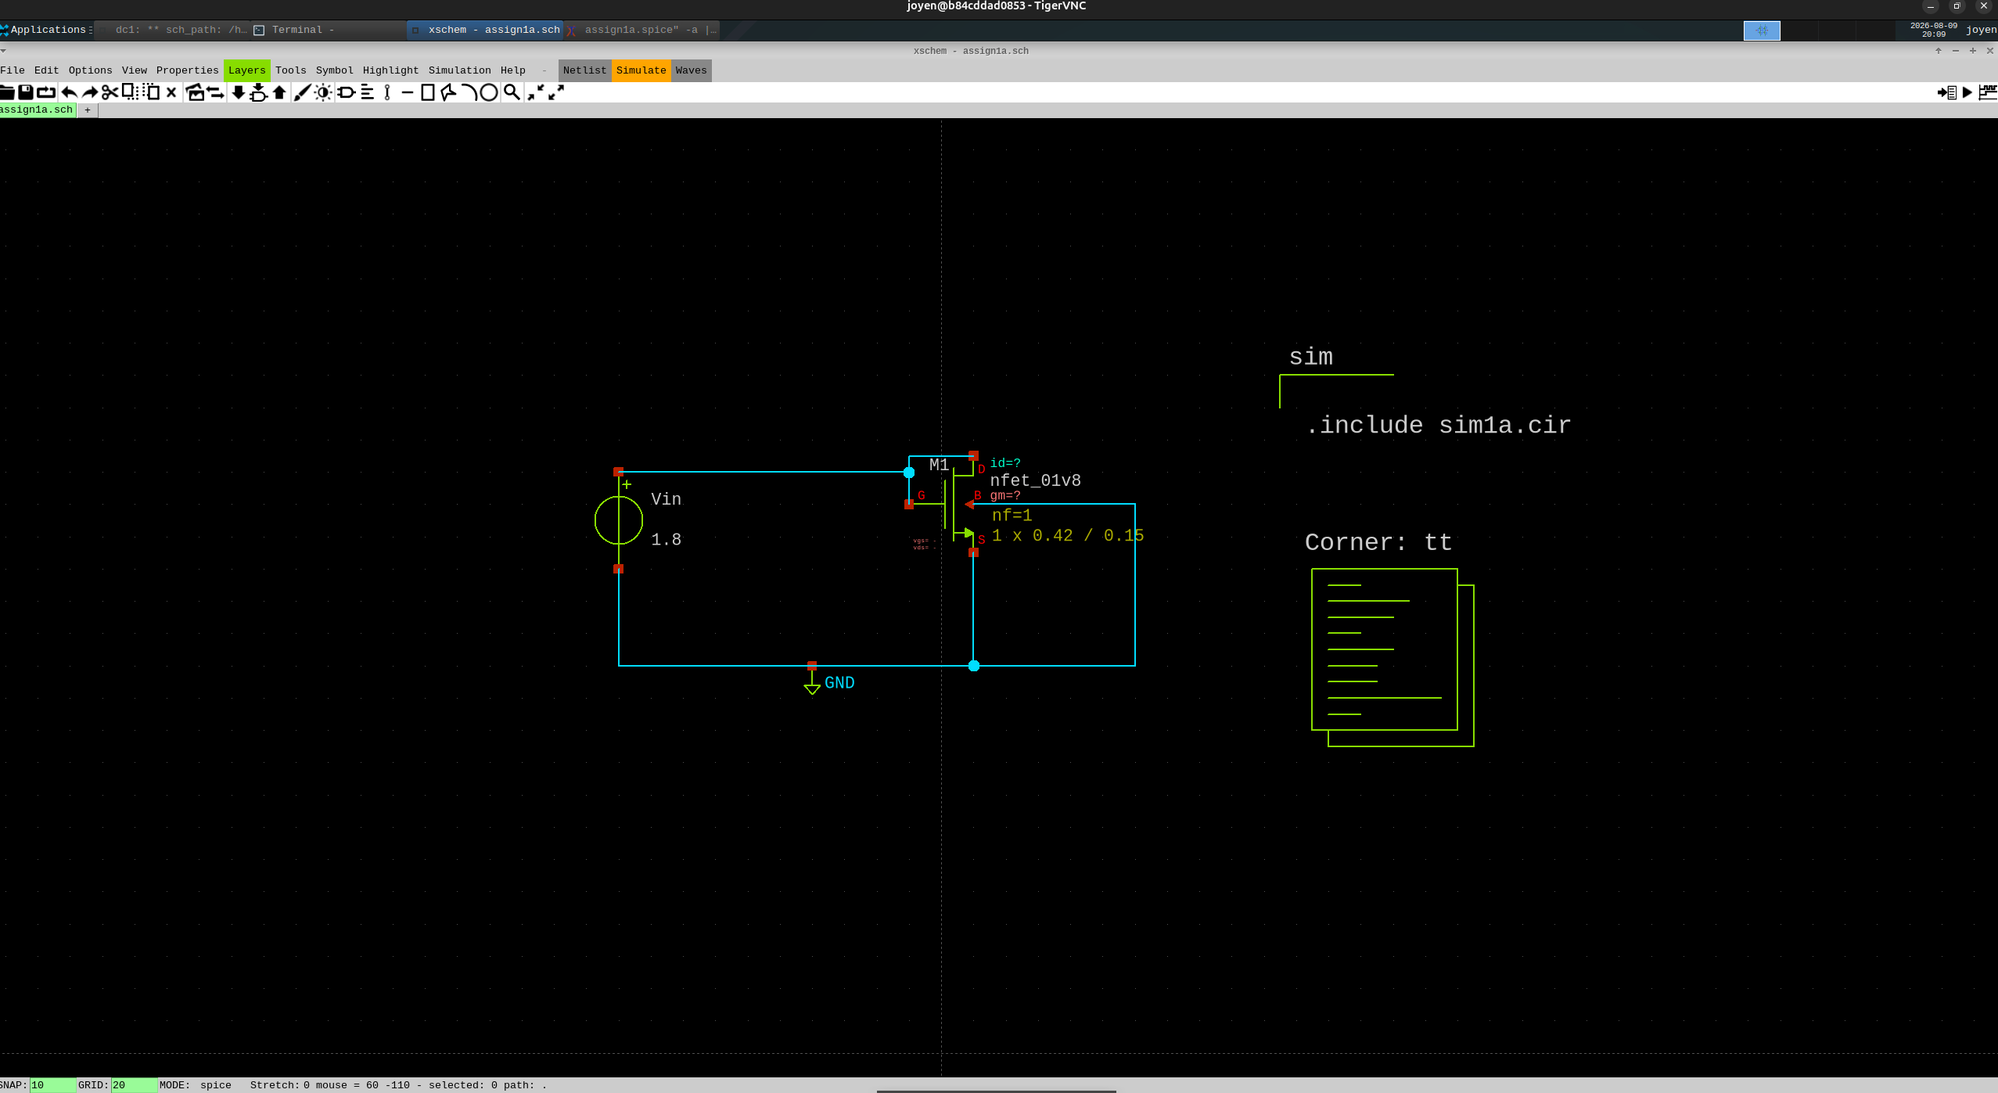
\includegraphics[width=0.8\textwidth]{figures/1a_schematic.png}
  \caption{Diode-connected nMOS used for the transfer-characteristic measurement.}
  \label{fig:1a-schematic}
\end{figure}

\subsubsection{Measurement}

The transfer characteristic and analytical comparison were generated by the following ngspice control script (\texttt{sim1a.cir}), included into \texttt{assign1a.spice} via \texttt{.include}:

\begin{verbatim}
.control
  dc Vin 0 1.8 0.01

  let w_val = 0.42u
  let l_val = 0.15u

  * Simulation data
  let ids_sim = -i(vin)

  * Analytical parameters
  let vgs = net1
  let vt_n = 0.7
  let meu_n = 0.025
  let cox_n = 8.34e-3
  let vsat_n = 8e4

  let vgt = max(0, vgs - vt_n)

  let EsatL = (vsat_n * l_val) / meu_n

  let vdsat = (vgt * EsatL) / (vgt + EsatL + 1e-12)

  let ids_anal = meu_n * cox_n * (w_val / l_val) * (vgt * vdsat - 0.5 * vdsat^2)

  * computing and printing the error
  let pct_error = abs((ids_sim - ids_anal) / (ids_sim + 1e-12)) * 100
  print mean(pct_error)

  plot ids_sim ids_anal vs vgs
.endc
\end{verbatim}

\begin{figure}[h]
  \centering
  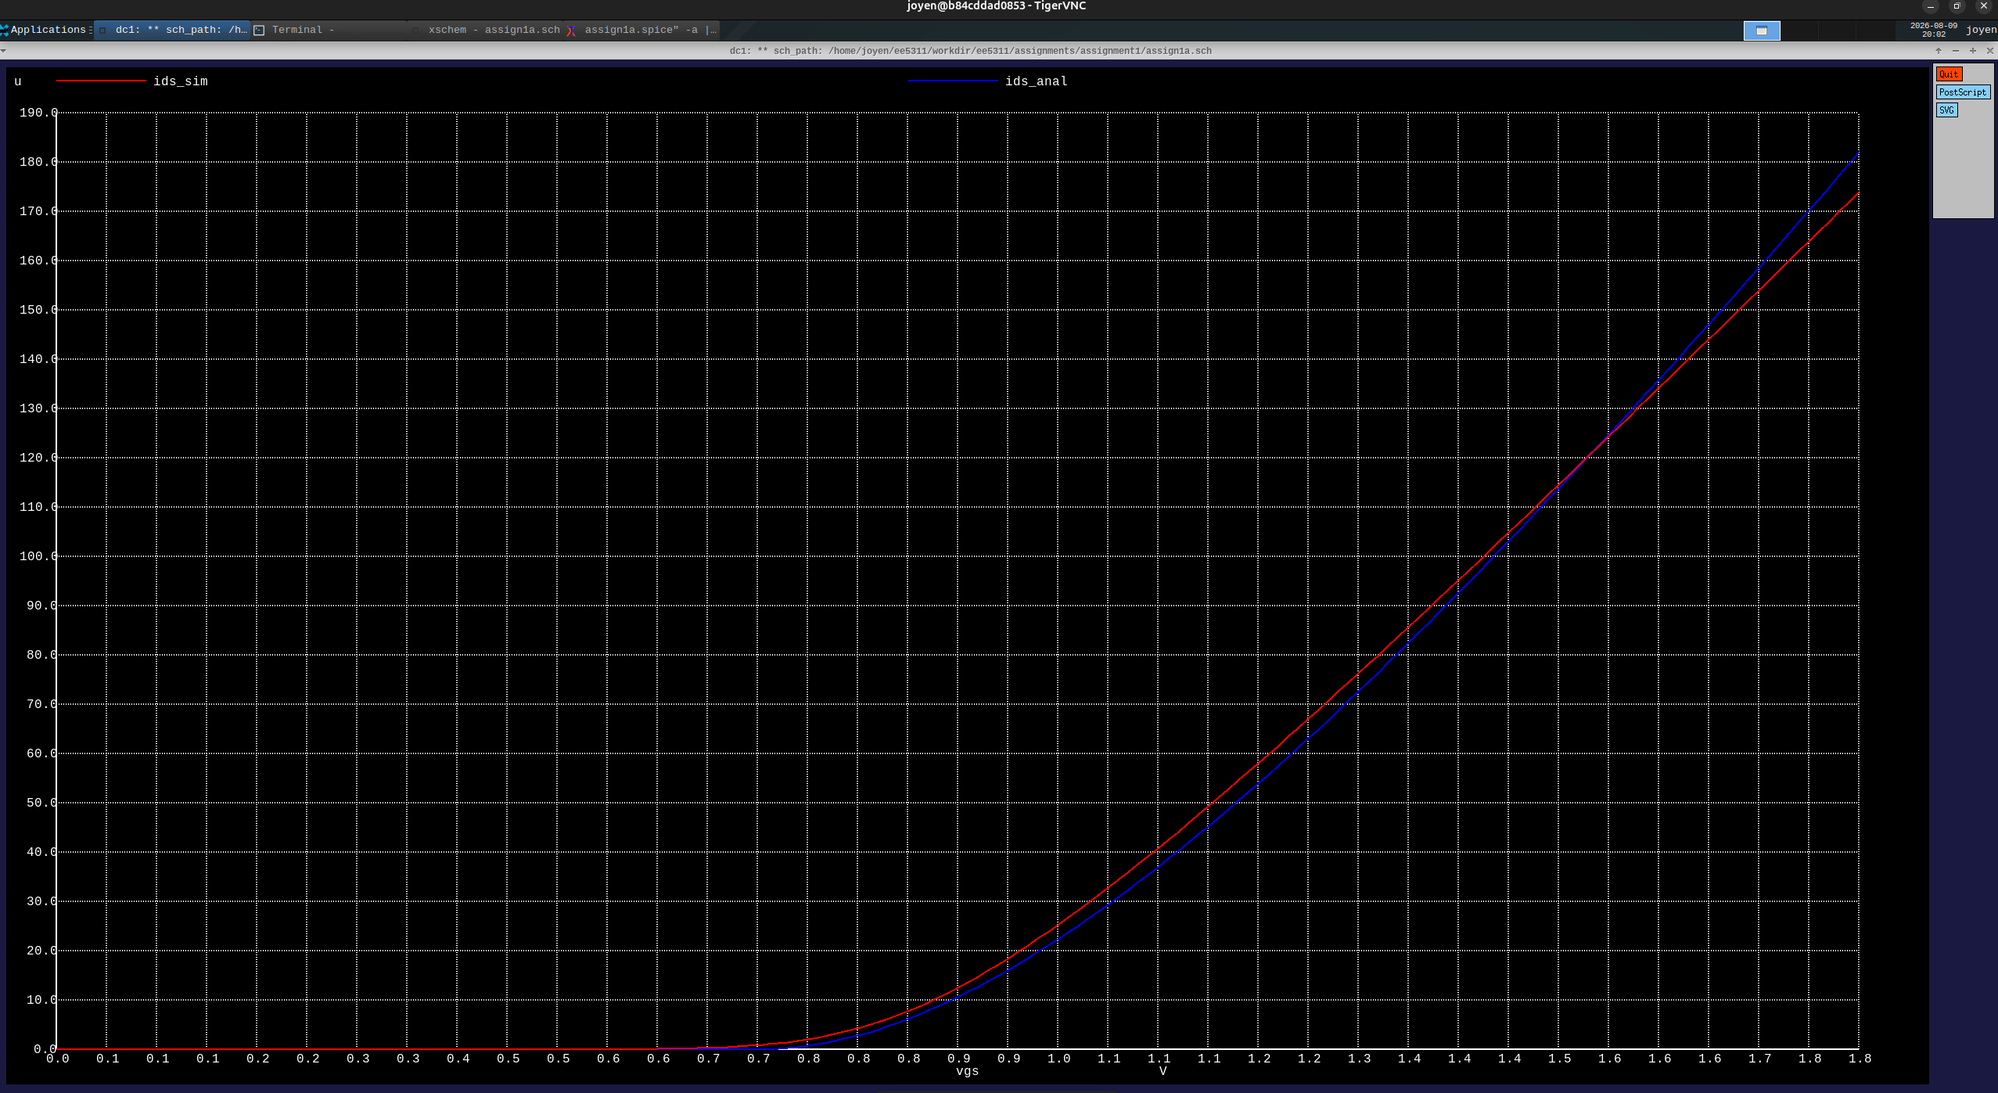
\includegraphics[width=0.95\textwidth]{figures/1a_plot.png}
  \caption{Simulated ($I_{ds,\text{sim}}$, red) vs.\ analytical ($I_{ds,\text{anal}}$, blue) $I_{ds}$--$V_{gs}$ transfer characteristic.}
  \label{fig:1a-measurement}
\end{figure}

Mean percentage error between the simulated and analytical curves: $\text{mean(pct\_error)} = 36.07$ \%.

\subsection{Part (b): nMOS Output Characteristics}

Connect the same nMOS transistor ($L = 0.15\ \mu\text{m}$, $W = 0.42\ \mu\text{m}$) with independent sources $V_{gs}$ at the gate and $V_{ds}$ at the drain (source and body grounded), and obtain the output characteristics for $V_{gs} = 0.6$ V, $1$ V, $1.4$ V, and $1.8$ V.

\begin{enumerate}
  \item Using Ngspice, sweep $V_{ds}$ from 0 to 1.8 V for each of the four fixed values of $V_{gs}$ (0.6 V, 1 V, 1.4 V, 1.8 V).
  \item Derive and plot the analytical output characteristic $I_{ds}$ vs.\ $V_{ds}$ for each $V_{gs}$, on the same axes as the simulated curves.
  \item Compute the mean percentage error between the simulated and analytical curves, for each of the four $V_{gs}$ values.
\end{enumerate}

\subsubsection{Calculation}

For each fixed $V_{gs}$, the same velocity-saturation model as Part (a) (Rabaey, Eq.~3.37--3.39) is used, now evaluated over the swept $V_{ds}$ instead of at a diode-connected operating point:
\[
V_{ov} = \max(0,\ V_{gs} - V_{Tn}), \qquad L\xi_c = \frac{v_{satn}\,L}{\mu_n}, \qquad V_{dsat} = \frac{V_{ov}\,(L\xi_c)}{V_{ov} + L\xi_c}
\]
The resistive-region current is evaluated at $\min(V_{ds},\,V_{dsat})$, which reduces to the ordinary triode expression for $V_{ds} < V_{dsat}$ and to the constant $I_{DSAT}$ of Eq.~(3.39) for $V_{ds} \geq V_{dsat}$ -- i.e., the current abruptly saturates, with no channel-length modulation:
\[
I_{ds,\text{anal}} = \mu_n C_{oxn} \frac{W}{L}\left[V_{ov}\min(V_{ds},V_{dsat}) - \frac{1}{2}\min(V_{ds},V_{dsat})^2\right]
\]

\subsubsection{Schematic}

\begin{figure}[h]
  \centering
  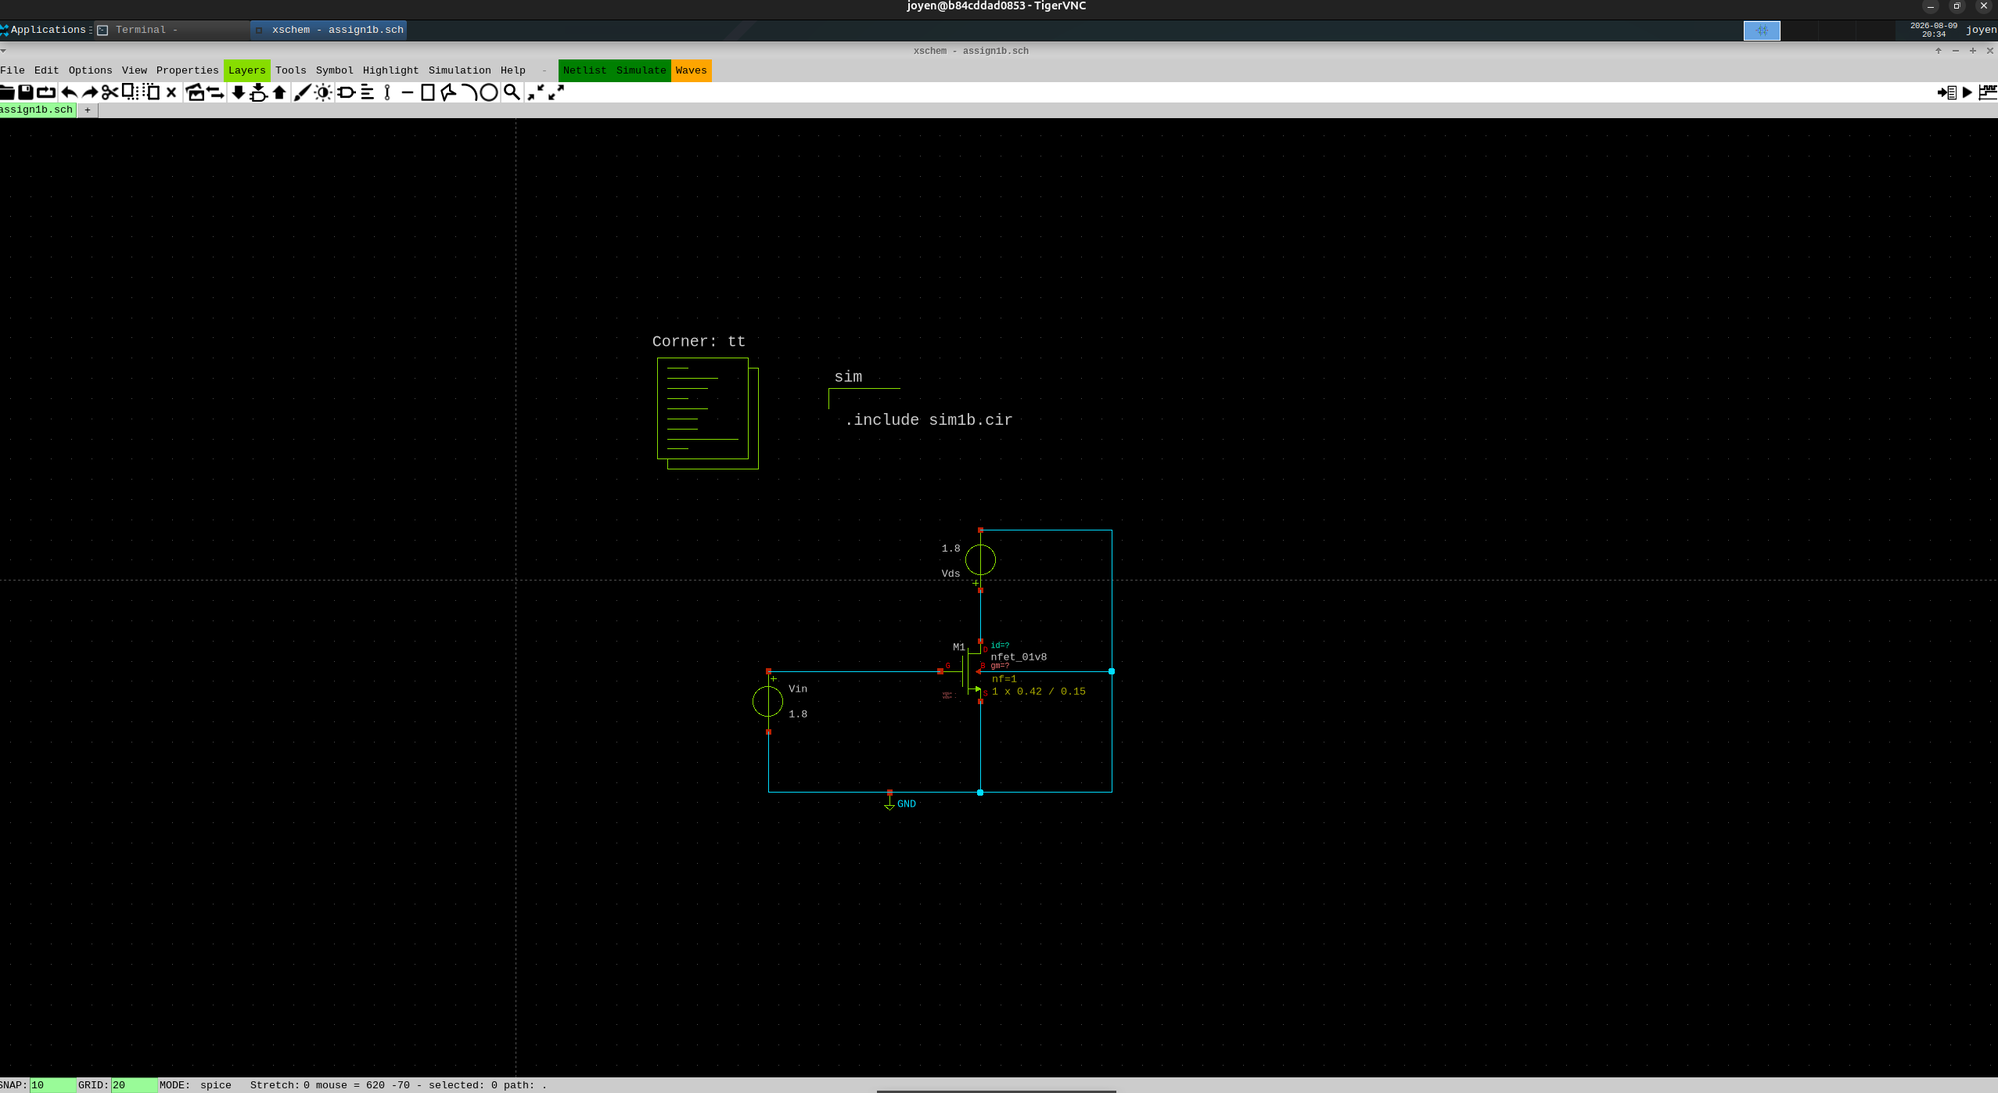
\includegraphics[width=0.8\textwidth]{figures/1b_schematic.png}
  \caption{nMOS with independent $V_{gs}$ and $V_{ds}$ sources used for the output-characteristic measurement.}
  \label{fig:1b-schematic}
\end{figure}

\subsubsection{Measurement}

The output characteristics and analytical comparison were generated by the following ngspice control script (\texttt{sim1b.cir}):

\begin{verbatim}
.control

* Process / device parameters (from Tutorial 1)
let vt_n     = 0.7
let mu_n     = 0.025
let cox_n    = 8.34e-3
let vsat_n   = 8e4
let w_val    = 0.42u
let l_val    = 0.15u
let EsatL    = (vsat_n * l_val) / mu_n

* Vgs values to sweep, one named constant per index (all defined before any
* analysis has run, so they stay globally visible from any later dc<N> plot)
let vgs1 = 0.6
let vgs2 = 1.0
let vgs3 = 1.4
let vgs4 = 1.8

foreach idx 1 2 3 4

  alter Vin = vgs$idx
  dc Vds 0 1.8 0.02

  let vds$idx      = v(net2)
  let ids_sim$idx  = -i(Vds)
  let vgt$idx      = max(0, vgs$idx - vt_n)
  let vdsat$idx    = (vgt$idx * EsatL) / (vgt$idx + EsatL + 1e-12)
  let vmin$idx     = min(vds$idx, vdsat$idx)
  let ids_anal$idx = mu_n * cox_n * (w_val / l_val) * (vgt$idx * vmin$idx - 0.5 * vmin$idx^2)
  let pct_error$idx = abs((ids_sim$idx - ids_anal$idx) / (ids_sim$idx + 1e-12)) * 100

  print mean(pct_error$idx)
end

plot Ids_sim_Vgs0_6V Ids_anal_Vgs0_6V Ids_sim_Vgs1_0V Ids_anal_Vgs1_0V \
     Ids_sim_Vgs1_4V Ids_anal_Vgs1_4V Ids_sim_Vgs1_8V Ids_anal_Vgs1_8V vs Vds_V
.endc
\end{verbatim}

\begin{figure}[h]
  \centering
  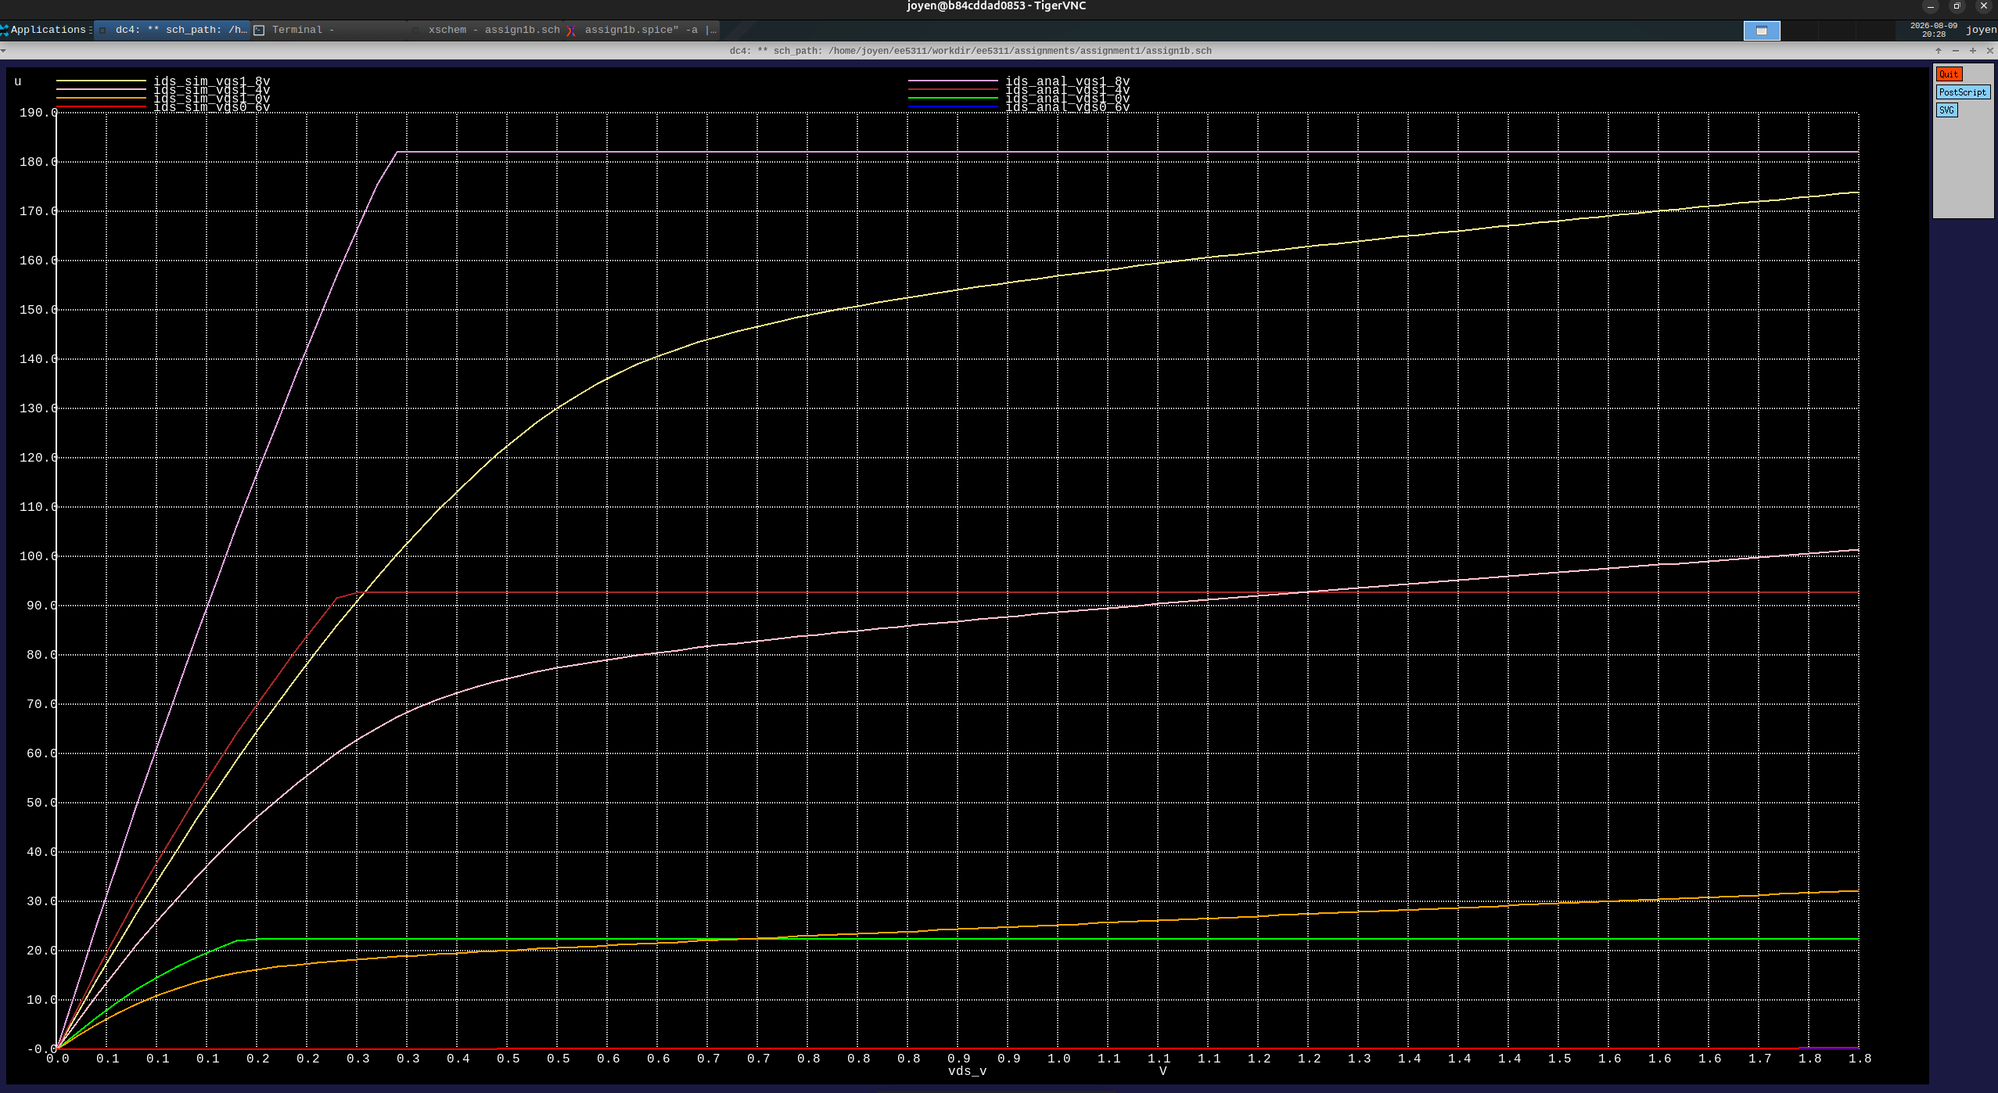
\includegraphics[width=0.95\textwidth]{figures/1b_plot.png}
  \caption{Simulated vs.\ analytical $I_{ds}$--$V_{ds}$ output characteristics for $V_{gs} = 0.6, 1.0, 1.4, 1.8$ V.}
  \label{fig:1b-measurement}
\end{figure}

\begin{table}[h]
  \centering
  \begin{tabular}{|c|c|}
    \hline
    $V_{gs}$ (V) & Mean \% error \\
    \hline
    0.6 & 98.90 \\
    1.0 & 18.01 \\
    1.4 & 15.54 \\
    1.8 & 30.51 \\
    \hline
  \end{tabular}
  \caption{Mean percentage error between simulated and analytical $I_{ds}$ for each $V_{gs}$.}
  \label{tab:1b-error}
\end{table}

\paragraph{Discussion.} The error is not uniform across $V_{gs}$, and the pattern is explained by where the analytical model's simplifying assumptions break down:
\begin{itemize}
  \item At $V_{gs}=0.6$~V (below the model's assumed $V_{Tn}=0.7$~V), the analytical model predicts $I_{ds}\approx 0$ throughout, since $V_{ov}=\max(0,-0.1)=0$. The simulated sky130 device is clearly already conducting substantially at this bias, indicating its actual threshold is somewhat lower than the textbook nominal value (and/or exhibits subthreshold conduction the model omits entirely). Whenever the analytical current is near zero while the simulated current is not, the percentage error is necessarily close to 100\% -- this is an artifact of operating near/below threshold, not a simulation error.
  \item At $V_{gs}=1.0$ and $1.4$~V, both curves track each other reasonably well (15--18\% error), which is a good result for a simple long-channel-plus-velocity-saturation model compared against a full sky130 BSIM simulation.
  \item At $V_{gs}=1.8$~V, the error rises again to $\sim\!31\%$ because the analytical model (per Eq.~3.38--3.39) saturates abruptly and stays flat past $V_{dsat}$, whereas the real device continues to gain current with $V_{ds}$ due to finite output resistance (channel-length modulation), an effect this simplified model deliberately excludes. This gap widens with overdrive/current level, consistent with what is observed.
\end{itemize}
Overall, this is a reproducible and expected outcome: the model matches well in the mid-overdrive region and diverges in well-understood ways near threshold and at high $V_{ds}$/$V_{gs}$, rather than indicating a setup mistake.

\subsection{Part (c): Effect of Transistor Size on Velocity Saturation}

Simulate $I_{ds}$ vs.\ $V_{ds}$ for $V_{gs} = V_{DD}$, for transistors of different $W/L$ while keeping the $W/L$ ratio constant and increasing the overall size. Note how the velocity saturation effect decreases as the overall channel length increases.

\subsubsection{Calculation}

$V_{gs}$ is fixed at $V_{DD}=1.8$~V, so the overdrive $V_{gt} = V_{DD} - V_{Tn} = 1.1$~V is the same constant for every size. Ten sizes are swept, scaling both $W$ and $L$ by the same integer multiplier $n = 1,\ldots,10$ from the base size ($W=0.42\,\mu\text{m}$, $L=0.15\,\mu\text{m}$), so $W/L = 2.8$ is held fixed throughout:
\[
W_n = n \times 0.42\ \mu\text{m}, \qquad L_n = n \times 0.15\ \mu\text{m}
\]
For each $L_n$, the same Eq.~(3.37)--(3.38) used in Parts (a)/(b) gives the critical-field length $L_n\xi_c$ and the saturation voltage:
\[
L_n\xi_c = \frac{v_{satn}\,L_n}{\mu_n}, \qquad V_{DSAT,n} = \frac{V_{gt}\,(L_n\xi_c)}{V_{gt} + L_n\xi_c}
\]
As $L_n \to \infty$, $L_n\xi_c \to \infty$ and $V_{DSAT,n} \to V_{gt}$ -- the ordinary long-channel saturation voltage, with no velocity-saturation compression. This motivates a direct measure of the velocity-saturation effect: the fractional shortfall of $V_{DSAT,n}$ below the ideal long-channel value $V_{gt}$,
\[
\text{VelSatEffect}_n = 1 - \frac{V_{DSAT,n}}{V_{gt}} = \frac{V_{gt}}{V_{gt} + L_n\xi_c}
\]
which is 1 in the limit of very short channels (maximal compression) and decreases monotonically to 0 as $L_n$ grows (no compression, long-channel limit). Unlike a ratio of simulated to ideal \emph{current}, this metric is derived purely from Eq.~(3.38) and is not affected by channel-length modulation or other second-order effects not modeled by this framework.

\begin{table}[h]
  \centering
  \begin{tabular}{|c|c|c|c|}
    \hline
    $n$ & $L_n$ ($\mu$m) & $V_{DSAT,n}$ (V) & VelSatEffect$_n$ \\
    \hline
    1  & 0.15 & 0.334 & 0.696 \\
    2  & 0.30 & 0.513 & 0.534 \\
    3  & 0.45 & 0.624 & 0.433 \\
    4  & 0.60 & 0.699 & 0.364 \\
    5  & 0.75 & 0.754 & 0.314 \\
    6  & 0.90 & 0.796 & 0.276 \\
    7  & 1.05 & 0.829 & 0.247 \\
    8  & 1.20 & 0.855 & 0.223 \\
    9  & 1.35 & 0.877 & 0.203 \\
    10 & 1.50 & 0.895 & 0.186 \\
    \hline
  \end{tabular}
  \caption{Predicted $V_{DSAT,n}$ and velocity-saturation effect for each of the 10 sizes ($V_{gt}=1.1$~V fixed).}
  \label{tab:1c-vdsat}
\end{table}

\subsubsection{Schematic}

\begin{figure}[h]
  \centering
  % TODO: replace with the actual xschem screenshot:
  % 
\includegraphics[width=0.6\textwidth]{figures/1c_schematic.png}
  \fbox{\parbox{0.6\textwidth}{\centering\vspace{3cm}Insert screenshot of \texttt{assign1c.sch} here\vspace{3cm}}}
  \caption{nMOS with gate fixed at $V_{DD}$ and drain swept, $W$ and $L$ parametrized for the size sweep.}
  \label{fig:1c-schematic}
\end{figure}

\subsubsection{Measurement}

The size sweep is implemented in \texttt{sim1c.cir} using ngspice's \texttt{.param}/\texttt{alterparam}/\texttt{reset}/\texttt{run} mechanism, looping the size multiplier $n=1,\ldots,10$:

\begin{verbatim}
.param Width = 0.42
.param Length = 0.15
.dc Vds 0 1.8 0.01
.control

let vt_n   = 0.7
let mu_n   = 0.025
let vsat_n = 8e4
let vgt    = 1.8 - vt_n

let index = 1
while index <= 10
    let newW = index * 0.42
    let newL = index * 0.15
    alterparam Width = $&newW
    alterparam Length = $&newL
    reset
    run

    let L_m        = newL * 1u
    let EsatL      = (vsat_n * L_m) / mu_n
    let vdsat_pred = (vgt * EsatL) / (vgt + EsatL)
    let velsat_effect = 1 - (vdsat_pred / vgt)

    let Vdsat_vs_L[index-1]        = vdsat_pred
    let VelSatEffect_vs_L[index-1] = velsat_effect
    let L_vec[index-1]             = newL

    let index = index + 1
end

plot $cache vs Vds_axis xlabel Vds_V ylabel Ids_A
plot VelSatEffect_vs_L vs L_vec xlabel L_um ylabel VelSatEffect
.endc
\end{verbatim}

\begin{figure}[h]
  \centering
  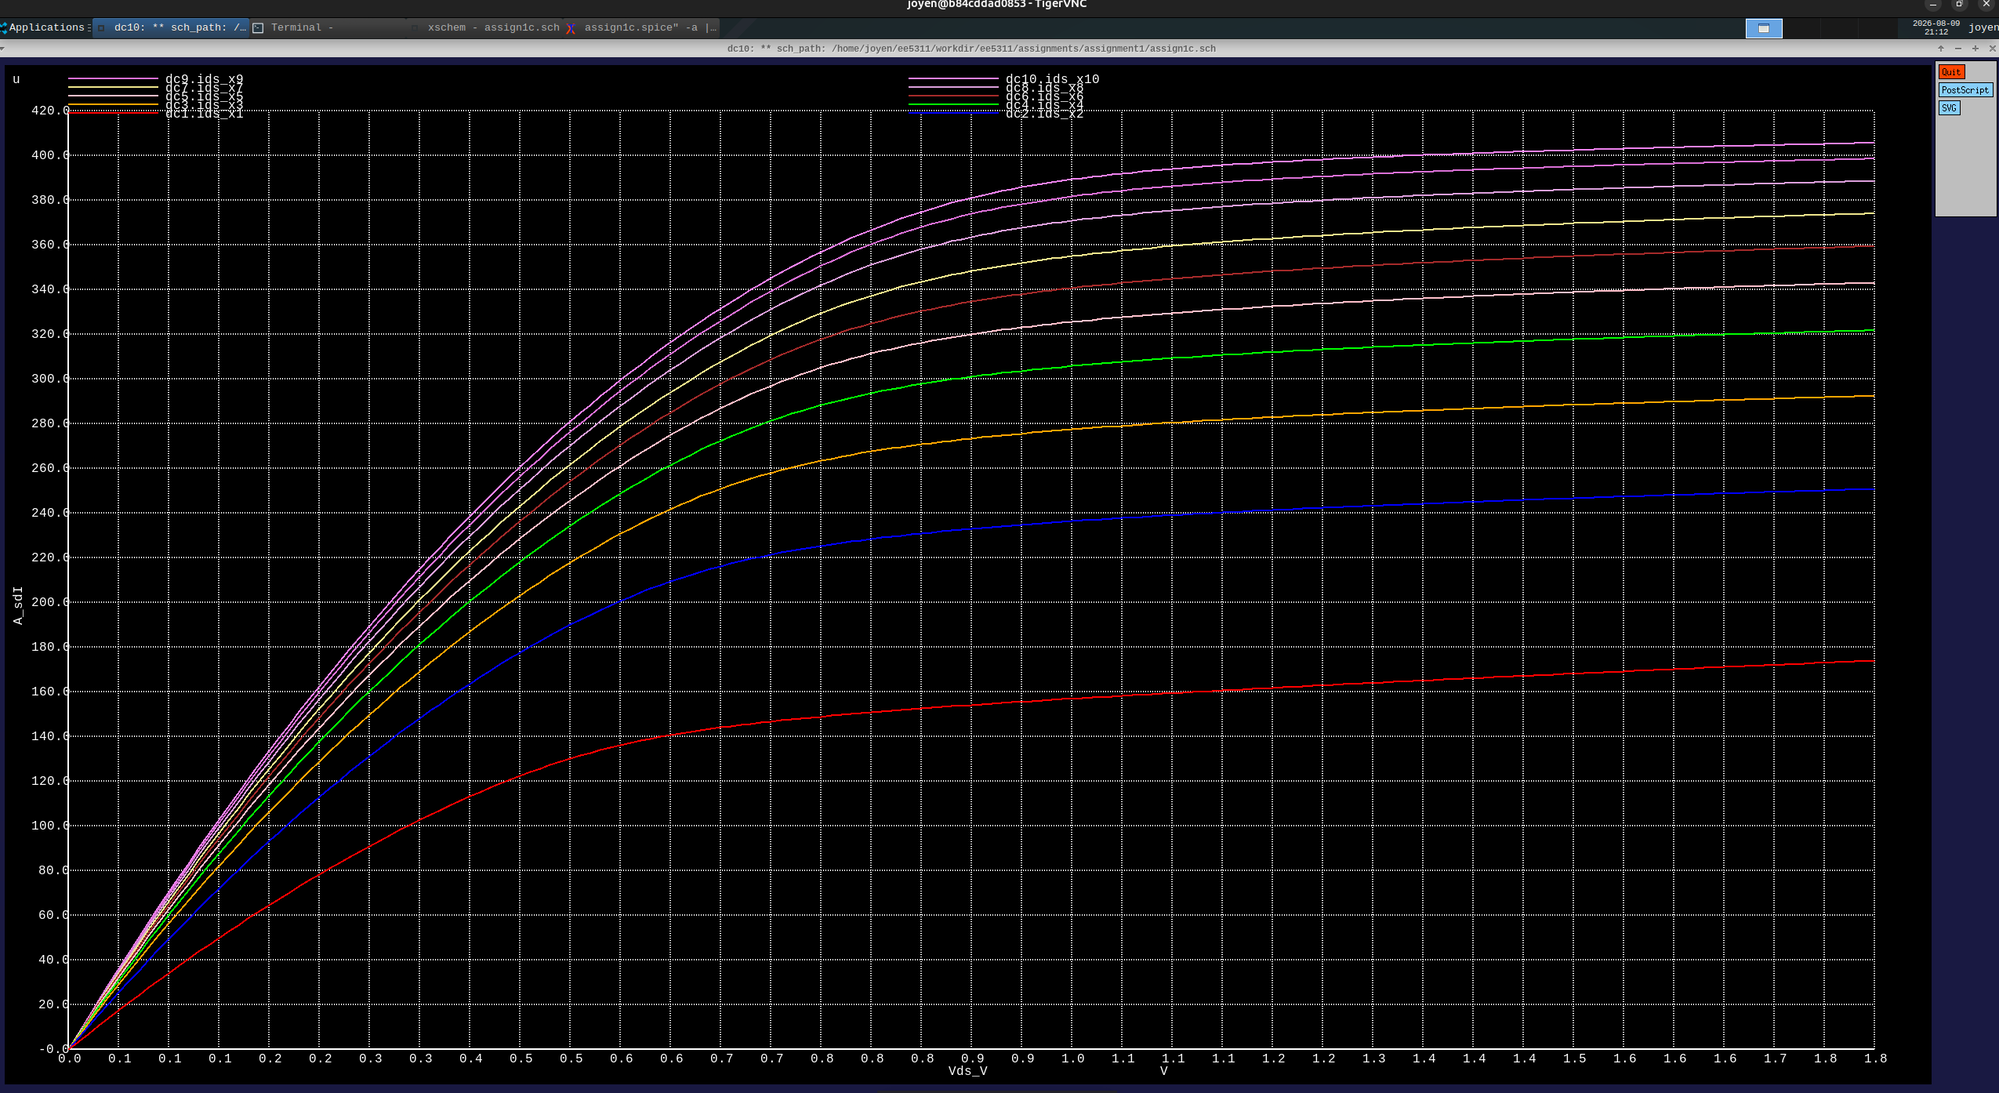
\includegraphics[width=0.95\textwidth]{figures/1c_iv_family.png}
  \caption{Simulated $I_{ds}$--$V_{ds}$ family of curves at $V_{gs}=V_{DD}$ for all 10 sizes (W/L ratio held at 2.8). Curves flatten later, and reach a higher current, as size increases.}
  \label{fig:1c-iv-family}
\end{figure}

\begin{figure}[h]
  \centering
  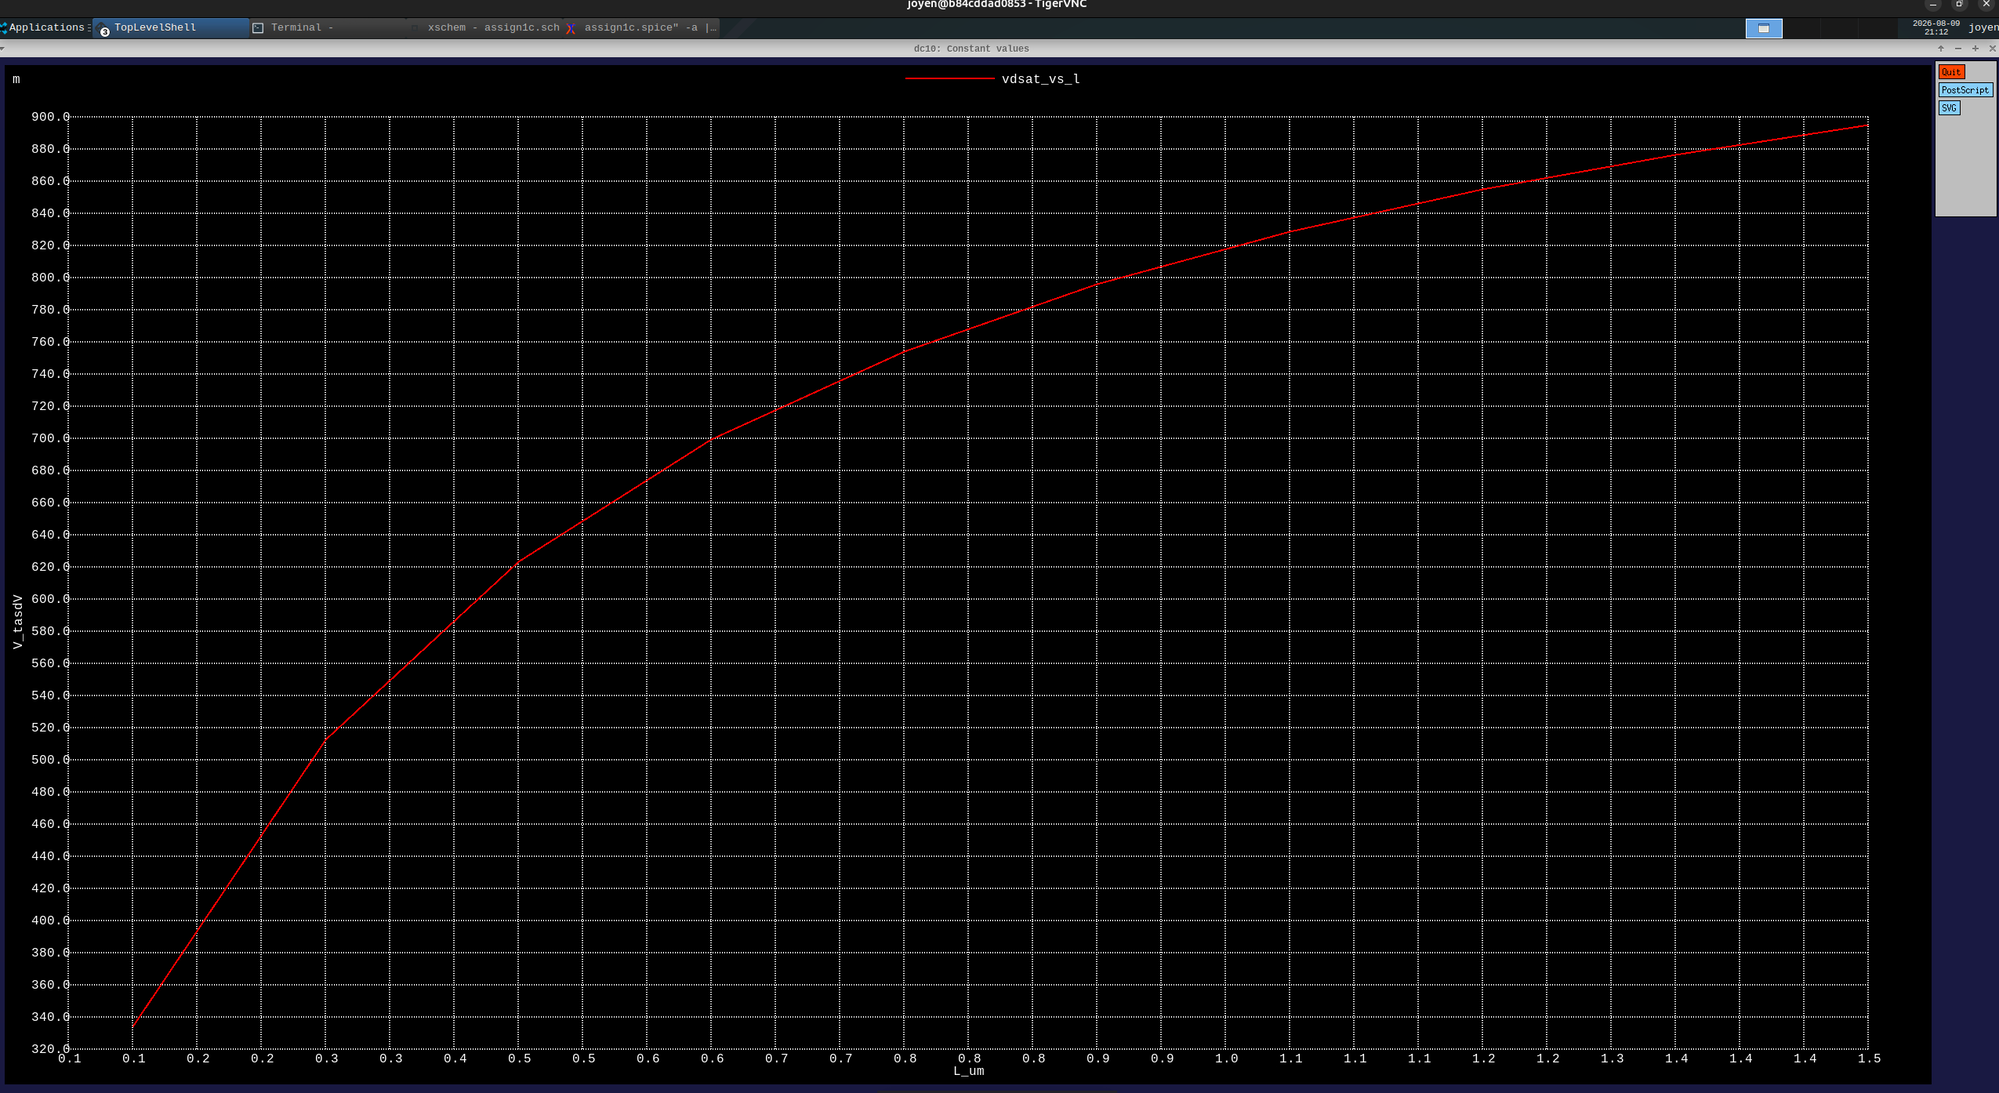
\includegraphics[width=0.8\textwidth]{figures/1c_vdsat_vs_L.png}
  \caption{Predicted $V_{DSAT}$ vs.\ channel length $L$: rises from 0.334~V toward the long-channel limit $V_{gt}=1.1$~V as $L$ grows.}
  \label{fig:1c-vdsat}
\end{figure}

\begin{figure}[h]
  \centering
  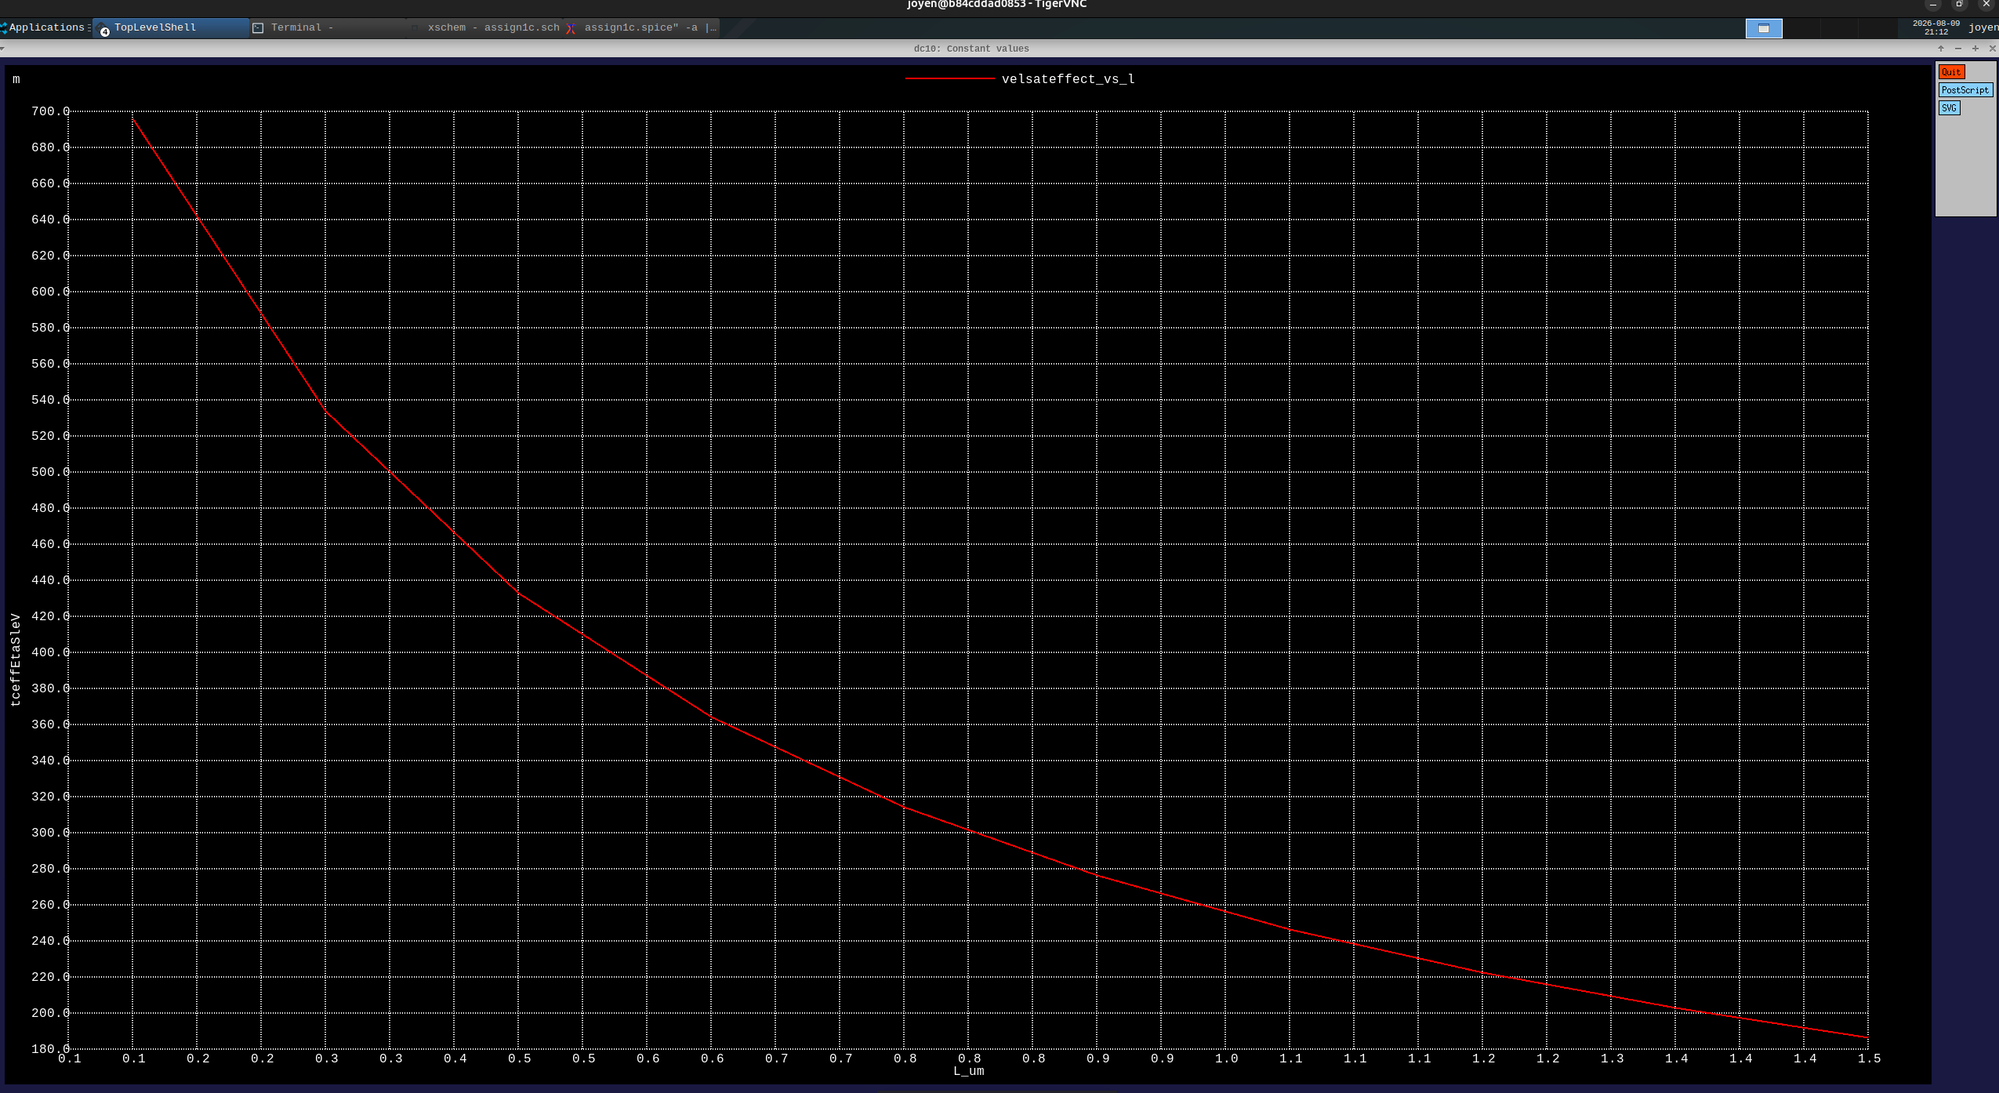
\includegraphics[width=0.8\textwidth]{figures/1c_velsateffect_vs_L.png}
  \caption{Velocity-saturation effect ($1 - V_{DSAT}/V_{gt}$) vs.\ channel length $L$: decreases monotonically from 0.696 (smallest size) to 0.186 (largest size).}
  \label{fig:1c-velsateffect}
\end{figure}

\paragraph{Discussion.} Figure~\ref{fig:1c-iv-family} shows the required simulated $I_{ds}$--$V_{ds}$ family: as the device size increases (constant $W/L=2.8$), the curves saturate at a noticeably later $V_{ds}$ and reach a higher current level. This is the qualitative signature asked for -- but to quantify it, Figures~\ref{fig:1c-vdsat} and \ref{fig:1c-velsateffect} isolate the effect directly from Eq.~(3.38): $V_{DSAT}$ climbs steadily toward the long-channel value $V_{gt}=1.1$~V as $L$ grows (Table~\ref{tab:1c-vdsat}), and the velocity-saturation effect metric falls monotonically from $0.696$ at the smallest size to $0.186$ at the largest -- a nearly $4\times$ reduction. Physically, $V_{DSAT}$ is compressed below $V_{gt}$ when the critical-field length $L\xi_c = v_{satn}L/\mu_n$ is comparable to or smaller than $V_{gt}$ (short channel, carriers hit the velocity-saturation limit before reaching the ideal pinch-off voltage); as $L$ increases, $L\xi_c$ grows linearly and eventually dominates $V_{gt}$, so the device recovers ordinary long-channel behavior and the compression -- i.e., the velocity-saturation effect -- vanishes.

\section{Problem 2}

\subsection{Part (a): pMOS Transfer Characteristics}

Consider a pMOS transistor with $L = 0.15\ \mu\text{m}$ and $W = 0.42\ \mu\text{m}$, connected in a diode-connected configuration: the gate and drain are tied together to a swept node $V_{in}$, the source and body are tied to $V_{DD}=1.8$~V, and the drain current $I_{sd}$ flows from $V_{DD}$ (through source and body) into the drain/gate node.

\begin{enumerate}
  \item Determine whether the transistor operates in the saturation or linear region for this connection.
  \item Using Ngspice, obtain the simulated transfer characteristic $I_{sd}$ vs.\ $V_{sg}$ by sweeping $V_{in}$ from $V_{DD}$ down to 0 V.
  \item Derive and plot the analytical transfer characteristic on the same axes, using the velocity-saturation drain current model.
  \item Compute the mean percentage error between the simulated and analytical curves.
\end{enumerate}

\subsubsection{Calculation}

This is the exact mirror of Part 1(a), with the rails and device type swapped: source and body sit at $V_{DD}$ instead of ground, and gate/drain are diode-connected to the swept node instead of source/body. Since gate and drain are tied together, $V_{sd} = V_{sg}$ at every point along the sweep. Once the device turns on ($V_{sg} > V_{Tp}$), the overdrive $V_{sgt} = V_{sg} - |V_{Tp}| \geq V_{SDSAT}$ (with equality only as $V_{Tp}\to0$), so $V_{sd} = V_{sg} > V_{sgt} \geq V_{SDSAT}$ always holds -- the diode-connected pMOS is therefore biased in \textbf{saturation} for the entire range where it conducts, same as the nMOS case.

The analytical drain current uses the same velocity-saturation model of Rabaey, \emph{Digital Integrated Circuits}, 2nd ed., p.~100, with the nMOS quantities replaced by their pMOS counterparts ($\mu_n\to\mu_p$, $v_{satn}\to v_{satp}$, $V_{Tn}\to|V_{Tp}|$, $C_{oxn}\to C_{oxp}$):
\[
\xi_c = \frac{v_{satp}}{\mu_p} \tag{3.37, pMOS}
\]
\[
V_{SDSAT} = L\,\xi_c = \frac{L\,v_{satp}}{\mu_p} \tag{3.38, pMOS}
\]
\[
I_{SDSAT} = \mu_p C_{oxp} \frac{W}{L}\left(V_{sgt}\,V_{SDSAT} - \frac{1}{2}V_{SDSAT}^2\right) \tag{3.39, pMOS}
\]
with $V_{sgt} = \max(0,\ V_{sg}-|V_{Tp}|)$. As in \texttt{sim1a.cir}, \texttt{sim2a.cir} smooths the constant approximation $L\xi_c$ against the overdrive,
\[
V_{sdsat} = \frac{V_{sgt}\,(L\xi_c)}{V_{sgt}+L\xi_c},
\]
which reduces to the long-channel result $V_{sdsat}\to V_{sgt}$ for small overdrive and to Eq.~(3.38, pMOS) for large overdrive, and substitutes this into the Eq.~(3.39, pMOS)-form expression for $I_{sd,\text{anal}}$.

\subsubsection{Schematic}

\begin{figure}[h]
  \centering
  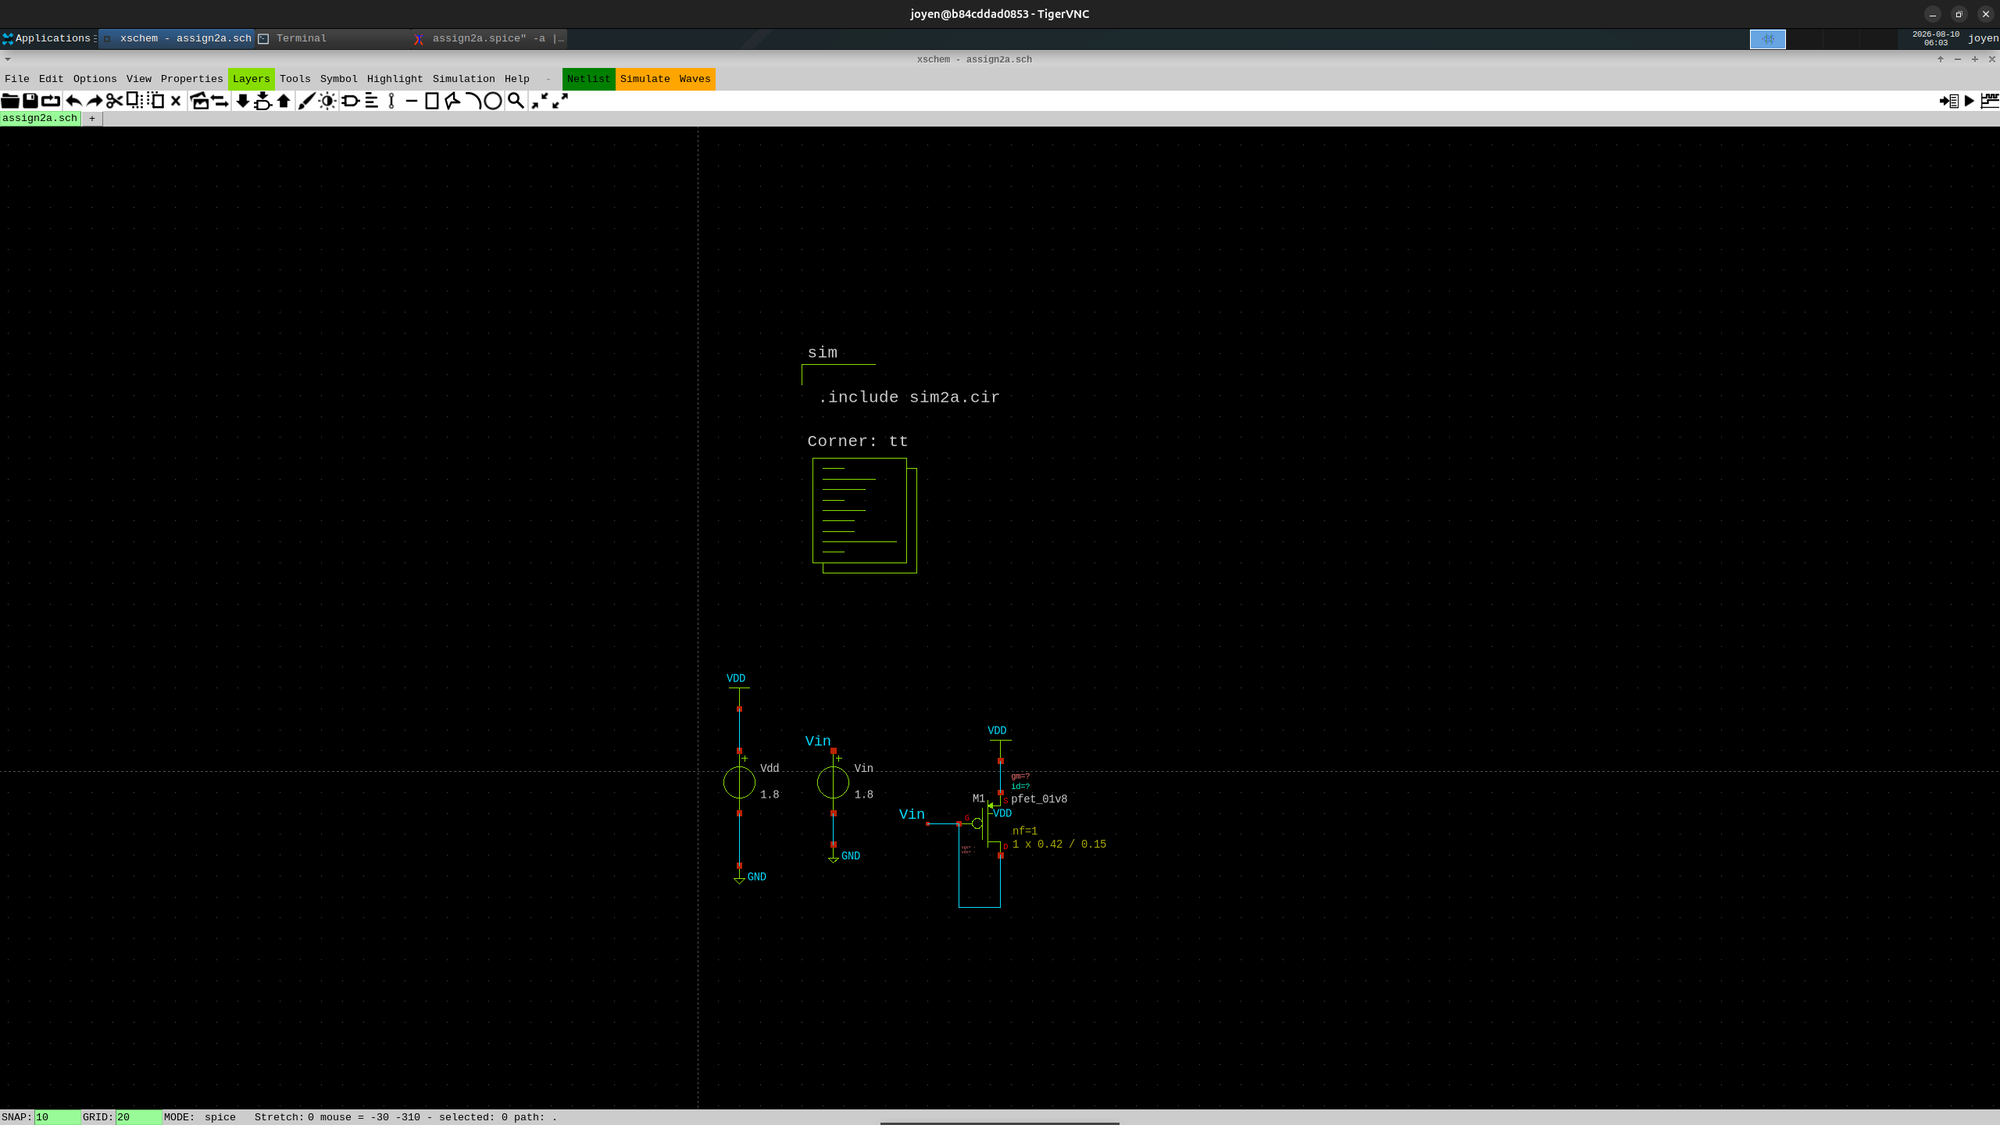
\includegraphics[width=0.8\textwidth]{figures/2a_schematic.png}
  \caption{Diode-connected pMOS used for the transfer-characteristic measurement: source and body tied to $V_{DD}$, gate and drain tied together to the swept node $V_{in}$.}
  \label{fig:2a-schematic}
\end{figure}

\subsubsection{Measurement}

The transfer characteristic and analytical comparison were generated by the following ngspice control script (\texttt{sim2a.cir}), included into \texttt{assign2a.spice} via \texttt{.include}:

\begin{verbatim}
.control
  dc Vin 1.8 0 -0.01

  let w_val = 0.42u
  let l_val = 0.15u

  * Simulation data (current flows into the Vin node from the transistor)
  let isd_sim = i(Vin)

  * Analytical parameters (pMOS, Tutorial 1)
  let vgs   = v(vin) - 1.8
  let vsg   = -vgs
  let vt_p  = 0.7
  let mu_p  = 0.009
  let cox_p = 8.16e-3
  let vsat_p = 3e4

  let vsgt = max(0, vsg - vt_p)

  let EsatL = (vsat_p * l_val) / mu_p

  let vsdsat = (vsgt * EsatL) / (vsgt + EsatL + 1e-12)

  let isd_anal = mu_p * cox_p * (w_val / l_val) * (vsgt * vsdsat - 0.5 * vsdsat^2)

  * computing and printing the error
  let pct_error = abs((isd_sim - isd_anal) / (isd_sim + 1e-12)) * 100
  print mean(pct_error)

  plot isd_sim isd_anal vs vsg
.endc
\end{verbatim}

\begin{figure}[h]
  \centering
  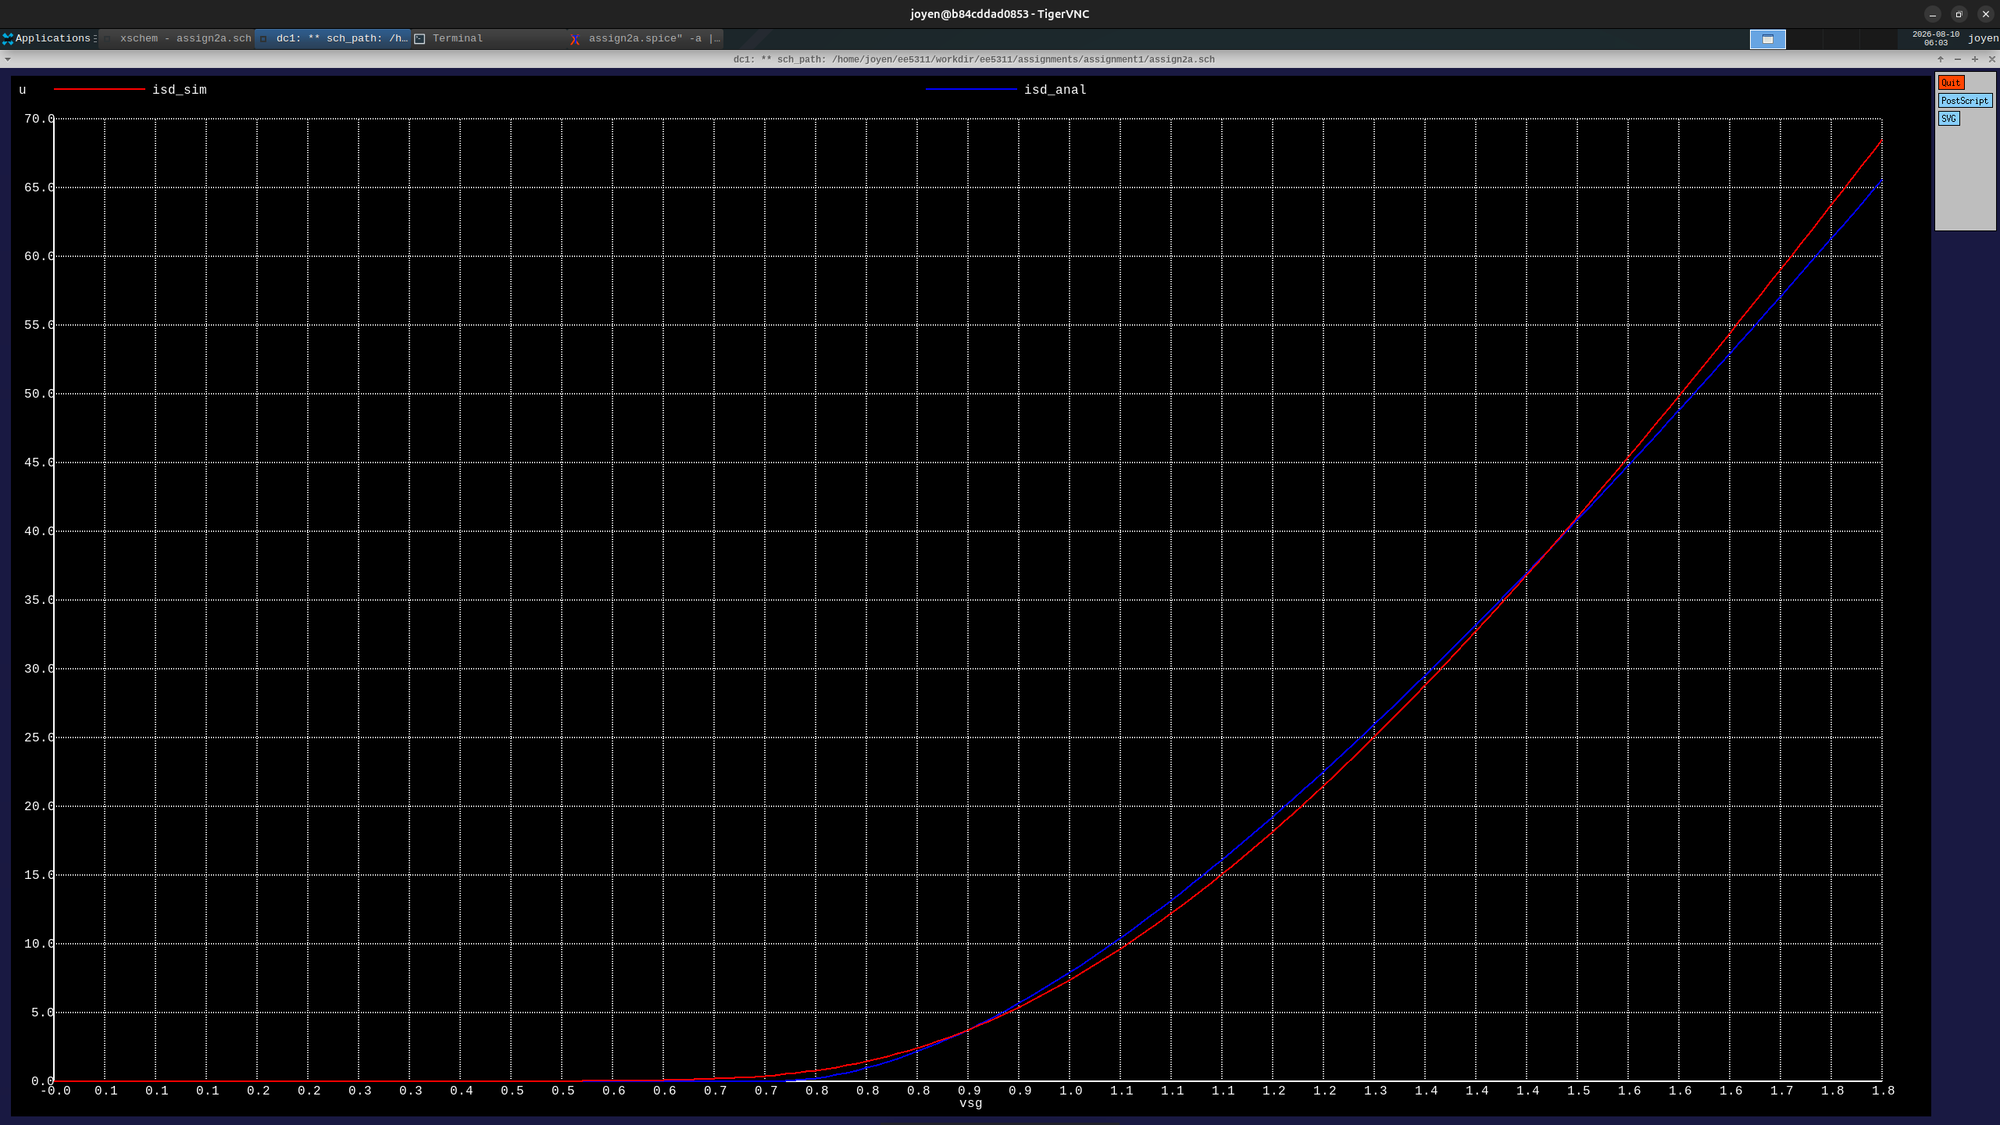
\includegraphics[width=0.95\textwidth]{figures/2a_plot.png}
  \caption{Simulated ($I_{sd,\text{sim}}$, red) vs.\ analytical ($I_{sd,\text{anal}}$, blue) $I_{sd}$--$V_{sg}$ transfer characteristic.}
  \label{fig:2a-measurement}
\end{figure}

Mean percentage error between the simulated and analytical curves: $\text{mean(pct\_error)} = 43.65$ \%.

\paragraph{Discussion.} The simulated and analytical $I_{sd}$--$V_{sg}$ curves track each other closely across the full sweep (Figure~\ref{fig:2a-measurement}), confirming that the same velocity-saturation model used for the nMOS in Part 1(a) applies equally well to the pMOS once the sign conventions and rail assignments are mirrored ($V_{gs}\to V_{sg}$, $I_{ds}\to I_{sd}$, source/body at $V_{DD}$ instead of ground). The lower mobility of holes ($\mu_p = 0.009\ \text{m}^2/\text{Vs}$ vs.\ $\mu_n=0.025\ \text{m}^2/\text{Vs}$) is why the pMOS delivers substantially less current than the nMOS for the same device size and overdrive -- the classic motivation for up-sizing pMOS transistors (larger $W$) relative to nMOS in real CMOS gates to balance pull-up/pull-down strength.

\subsection{Part (b): pMOS Output Characteristics}

Connect the same pMOS transistor ($L = 0.15\ \mu\text{m}$, $W = 0.42\ \mu\text{m}$) with independent sources at the gate and drain (source and body tied to $V_{DD}$), and obtain the output characteristics for $V_{sg} = 0.6$ V, $1$ V, $1.4$ V, and $1.8$ V.

\begin{enumerate}
  \item Using Ngspice, sweep $V_{sd}$ from 0 to 1.8 V for each of the four fixed values of $V_{sg}$ (0.6 V, 1 V, 1.4 V, 1.8 V).
  \item Derive and plot the analytical output characteristic $I_{sd}$ vs.\ $V_{sd}$ for each $V_{sg}$, on the same axes as the simulated curves.
  \item Compute the mean percentage error between the simulated and analytical curves, for each of the four $V_{sg}$ values.
\end{enumerate}

\subsubsection{Calculation}

Exact mirror of Part 1(b), with the pMOS quantities substituted in. For each fixed $V_{sg}$, the same velocity-saturation model as Part 2(a) (Rabaey, Eq.~3.37--3.39, pMOS form) is used, now evaluated over the swept $V_{sd}$ instead of at a diode-connected operating point:
\[
V_{sgt} = \max(0,\ V_{sg} - |V_{Tp}|), \qquad L\xi_c = \frac{v_{satp}\,L}{\mu_p}, \qquad V_{sdsat} = \frac{V_{sgt}\,(L\xi_c)}{V_{sgt} + L\xi_c}
\]
The resistive-region current is evaluated at $\min(V_{sd},\,V_{sdsat})$, which reduces to the ordinary triode expression for $V_{sd} < V_{sdsat}$ and to the constant $I_{SDSAT}$ of Eq.~(3.39, pMOS) for $V_{sd}\geq V_{sdsat}$ -- an abrupt saturation, with no channel-length modulation:
\[
I_{sd,\text{anal}} = \mu_p C_{oxp} \frac{W}{L}\left[V_{sgt}\min(V_{sd},V_{sdsat}) - \frac{1}{2}\min(V_{sd},V_{sdsat})^2\right]
\]

In the schematic, source and body are tied to $V_{DD}$ rather than ground, so the two independent sources set \emph{absolute} node voltages rather than $V_{sg}$/$V_{sd}$ directly: the gate source \texttt{Vin} must be set to $V_{DD}-V_{sg}$, and the drain source \texttt{Vds} is swept from $V_{DD}$ down to 0 so that $V_{sd}=V_{DD}-V(\texttt{vds})$ ascends from 0 to 1.8~V, matching the sweep direction used in Part 1(b).

\subsubsection{Schematic}

\begin{figure}[h]
  \centering
  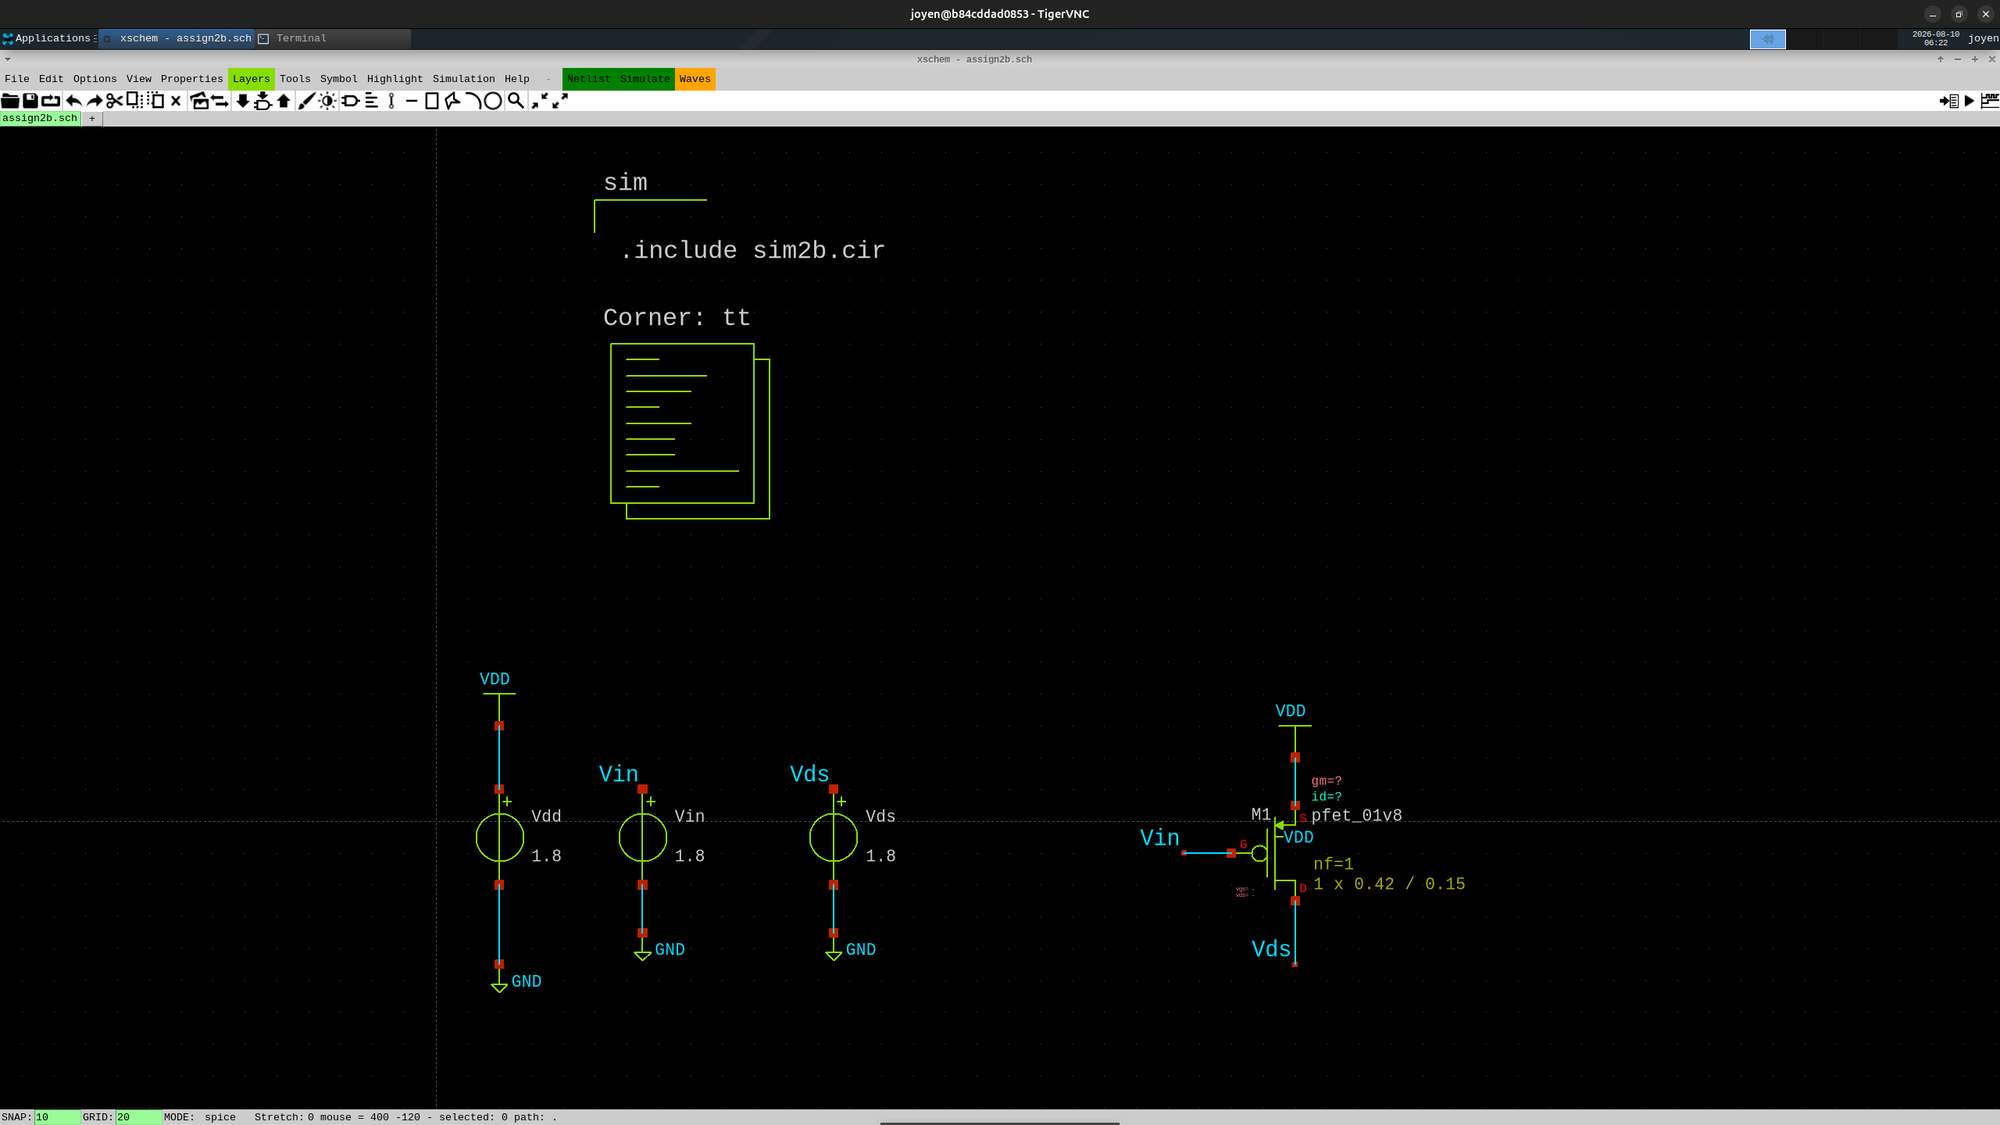
\includegraphics[width=0.8\textwidth]{figures/2b_schematic.png}
  \caption{pMOS with independent gate (\texttt{Vin}) and drain (\texttt{Vds}) sources, source/body tied to $V_{DD}$, used for the output-characteristic measurement.}
  \label{fig:2b-schematic}
\end{figure}

\subsubsection{Measurement}

The output characteristics and analytical comparison were generated by the following ngspice control script (\texttt{sim2b.cir}):

\begin{verbatim}
.control

* Process / device parameters (pMOS, Tutorial 1)
let vt_p     = 0.7
let mu_p     = 0.009
let cox_p    = 8.16e-3
let vsat_p   = 3e4
let w_val    = 0.42u
let l_val    = 0.15u
let EsatL    = (vsat_p * l_val) / mu_p

let vsg1 = 0.6
let vsg2 = 1.0
let vsg3 = 1.4
let vsg4 = 1.8

foreach idx 1 2 3 4

  alter Vin = 1.8 - vsg$idx
  dc Vds 1.8 0 -0.02

  let vsd$idx      = 1.8 - v(vds)
  let isd_sim$idx  = i(Vds)
  let vsgt$idx     = max(0, vsg$idx - vt_p)
  let vsdsat$idx   = (vsgt$idx * EsatL) / (vsgt$idx + EsatL + 1e-12)
  let vmin$idx     = min(vsd$idx, vsdsat$idx)
  let isd_anal$idx = mu_p * cox_p * (w_val / l_val) * (vsgt$idx * vmin$idx - 0.5 * vmin$idx^2)
  let pct_error$idx = abs((isd_sim$idx - isd_anal$idx) / (isd_sim$idx + 1e-12)) * 100

  print mean(pct_error$idx)
end

plot Isd_sim_Vsg0_6V Isd_anal_Vsg0_6V Isd_sim_Vsg1_0V Isd_anal_Vsg1_0V \
     Isd_sim_Vsg1_4V Isd_anal_Vsg1_4V Isd_sim_Vsg1_8V Isd_anal_Vsg1_8V vs Vsd_V
.endc
\end{verbatim}

\begin{figure}[h]
  \centering
  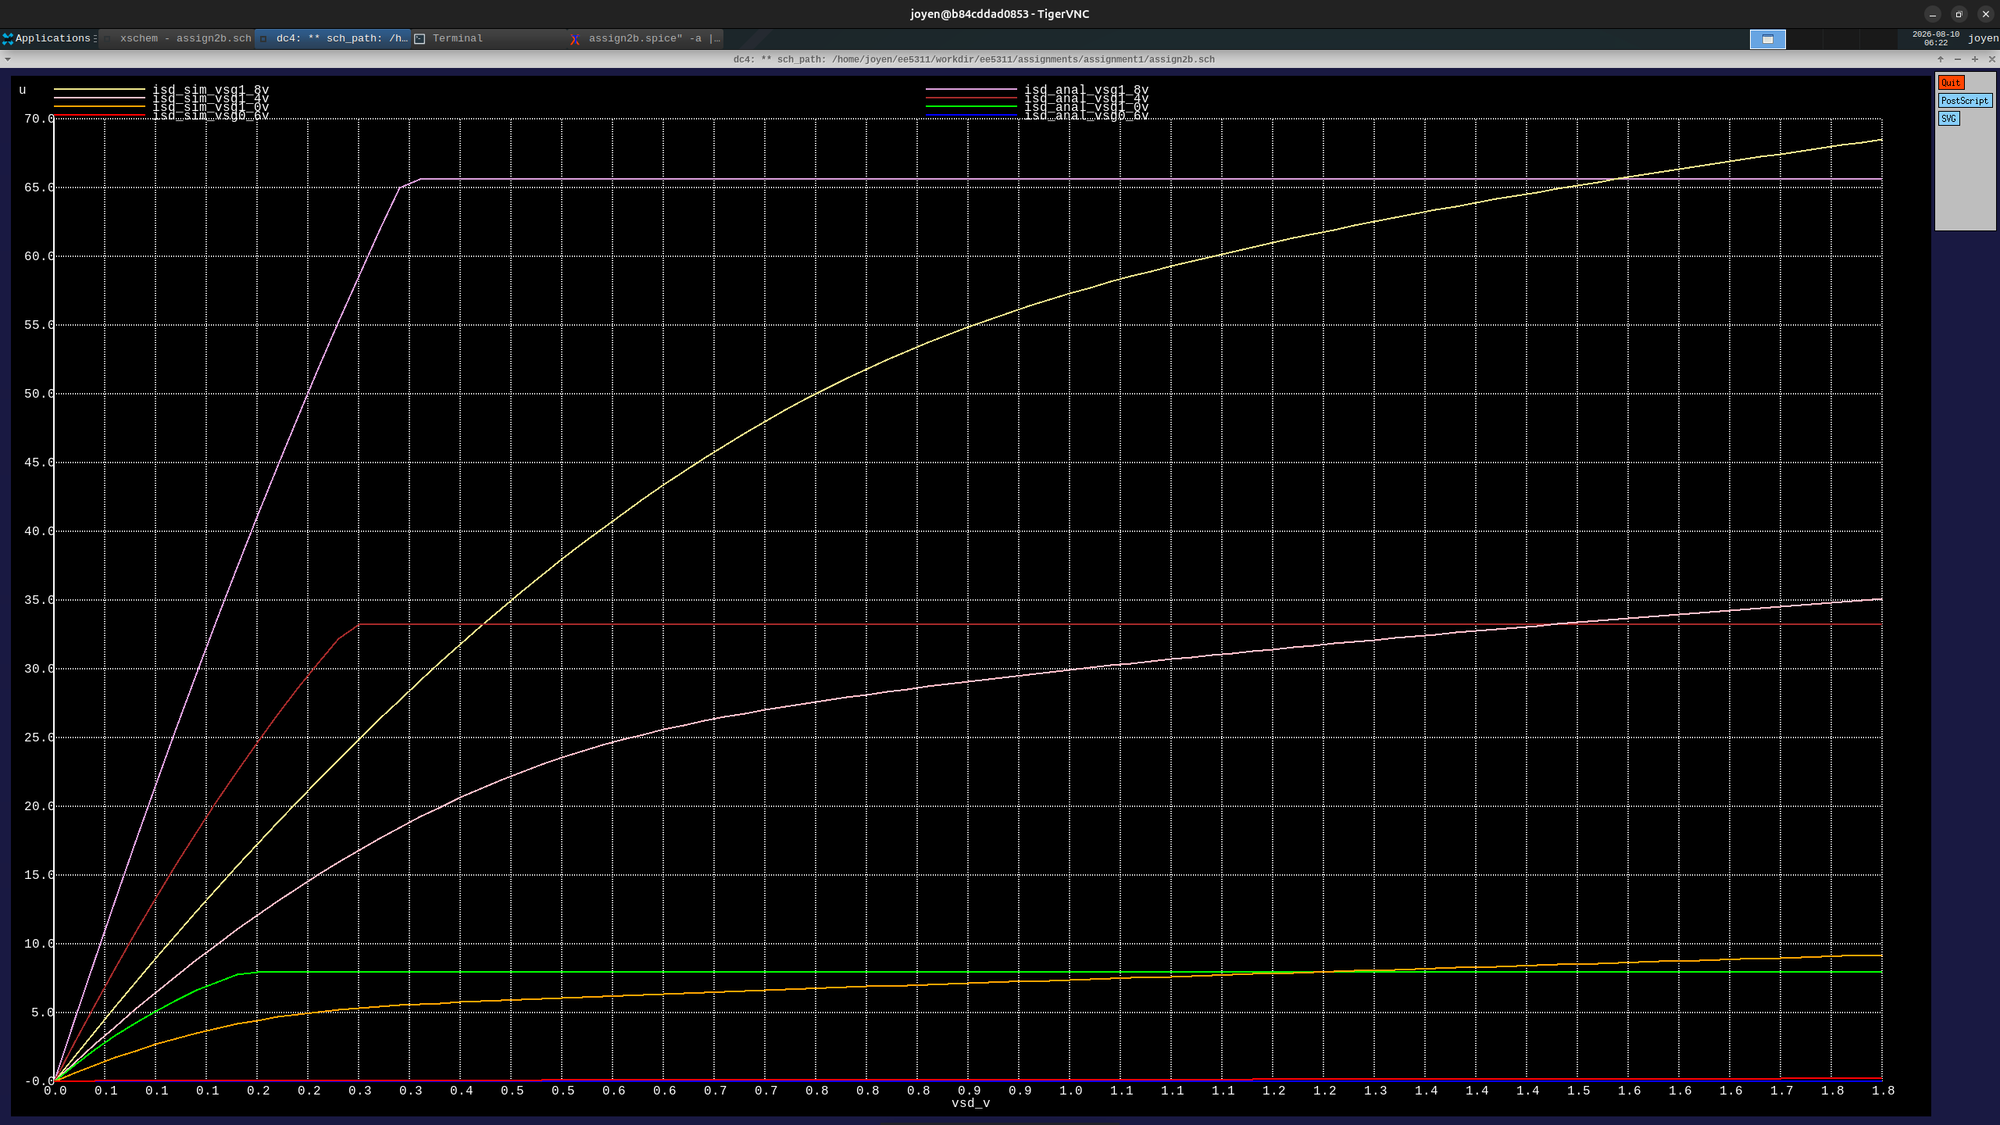
\includegraphics[width=0.95\textwidth]{figures/2b_plot.png}
  \caption{Simulated vs.\ analytical $I_{sd}$--$V_{sd}$ output characteristics for $V_{sg} = 0.6, 1.0, 1.4, 1.8$ V.}
  \label{fig:2b-measurement}
\end{figure}

\begin{table}[h]
  \centering
  \begin{tabular}{|c|c|}
    \hline
    $V_{sg}$ (V) & Mean \% error \\
    \hline
    0.6 & 98.90 \\
    1.0 & 24.57 \\
    1.4 & 31.56 \\
    1.8 & 45.79 \\
    \hline
  \end{tabular}
  \caption{Mean percentage error between simulated and analytical $I_{sd}$ for each $V_{sg}$.}
  \label{tab:2b-error}
\end{table}

\paragraph{Discussion.} The error pattern reproduces the same two artifacts seen in Part 1(b), for the same reasons:
\begin{itemize}
  \item At $V_{sg}=0.6$~V (below $|V_{Tp}|=0.7$~V), the analytical model predicts $I_{sd}\approx0$ since $V_{sgt}=\max(0,-0.1)=0$, while the simulated sky130 pMOS is already conducting somewhat -- so the percentage error is forced close to 100\%. This is identical, down to the reported value ($98.90\%$, matching Part 1(b)'s $V_{gs}=0.6$~V result exactly), confirming it is the same near-threshold/subthreshold artifact rather than a setup error.
  \item At $V_{sg}=1.0$ and $1.4$~V, the error is higher than the corresponding nMOS case ($24.57\%$/$31.56\%$ vs.\ $18.01\%$/$15.54\%$), and at $V_{sg}=1.8$~V it is again higher ($45.79\%$ vs.\ $30.51\%$). The larger mismatch is consistent with the pMOS's lower mobility and correspondingly smaller drive current: with $I_{sd}$ an order of magnitude smaller than $I_{ds}$ for the same overdrive, the same absolute deviation from channel-length modulation (which this simplified model excludes) represents a larger \emph{relative} error.
\end{itemize}
As in Part 1(b), this is a reproducible, physically-explained outcome rather than an indication of a wiring or model mistake.

\subsection{Part (c): Effect of Transistor Size on Velocity Saturation (pMOS)}

Simulate $I_{sd}$ vs.\ $V_{sd}$ for $V_{sg} = V_{DD}$, for pMOS transistors of different $W/L$ while keeping the $W/L$ ratio constant and increasing the overall size. Note how the velocity saturation effect decreases as the overall channel length increases, and compare against the nMOS result of Part 1(c).

\subsubsection{Calculation}

Exact mirror of Part 1(c). $V_{sg}$ is fixed at $V_{DD}=1.8$~V (gate held at 0~V absolute, since source/body sit at $V_{DD}$), so the overdrive $V_{sgt} = V_{DD} - |V_{Tp}| = 1.1$~V is the same constant for every size. Ten sizes are swept, scaling both $W$ and $L$ by the same integer multiplier $n=1,\ldots,10$ from the base size ($W=0.42\,\mu\text{m}$, $L=0.15\,\mu\text{m}$), so $W/L=2.8$ is held fixed throughout. For each $L_n$, Eq.~(3.37)--(3.38) (pMOS form) gives
\[
L_n\xi_{c,p} = \frac{v_{satp}\,L_n}{\mu_p}, \qquad V_{SDSAT,n} = \frac{V_{sgt}\,(L_n\xi_{c,p})}{V_{sgt}+L_n\xi_{c,p}}, \qquad \text{VelSatEffect}_n = 1-\frac{V_{SDSAT,n}}{V_{sgt}}
\]
As established in the Problem 2(a) discussion of Rabaey p.~68 (\emph{"the effects of velocity saturation are less pronounced [in pMOS] ... due to the higher critical field from the smaller hole mobility"}), $\xi_{c,p}=v_{satp}/\mu_p$ should be \emph{larger} than $\xi_{c,n}=v_{satn}/\mu_n$ for this process:
\[
\xi_{c,n} = \frac{8\times10^4}{0.025} = 3.2\times10^6\ \text{V/m}, \qquad \xi_{c,p} = \frac{3\times10^4}{0.009} = 3.33\times10^6\ \text{V/m}
\]
a $\sim\!4\%$ increase, predicting a correspondingly smaller VelSatEffect for the pMOS than the nMOS at matching $L$.

\subsubsection{Schematic}

\begin{figure}[h]
  \centering
  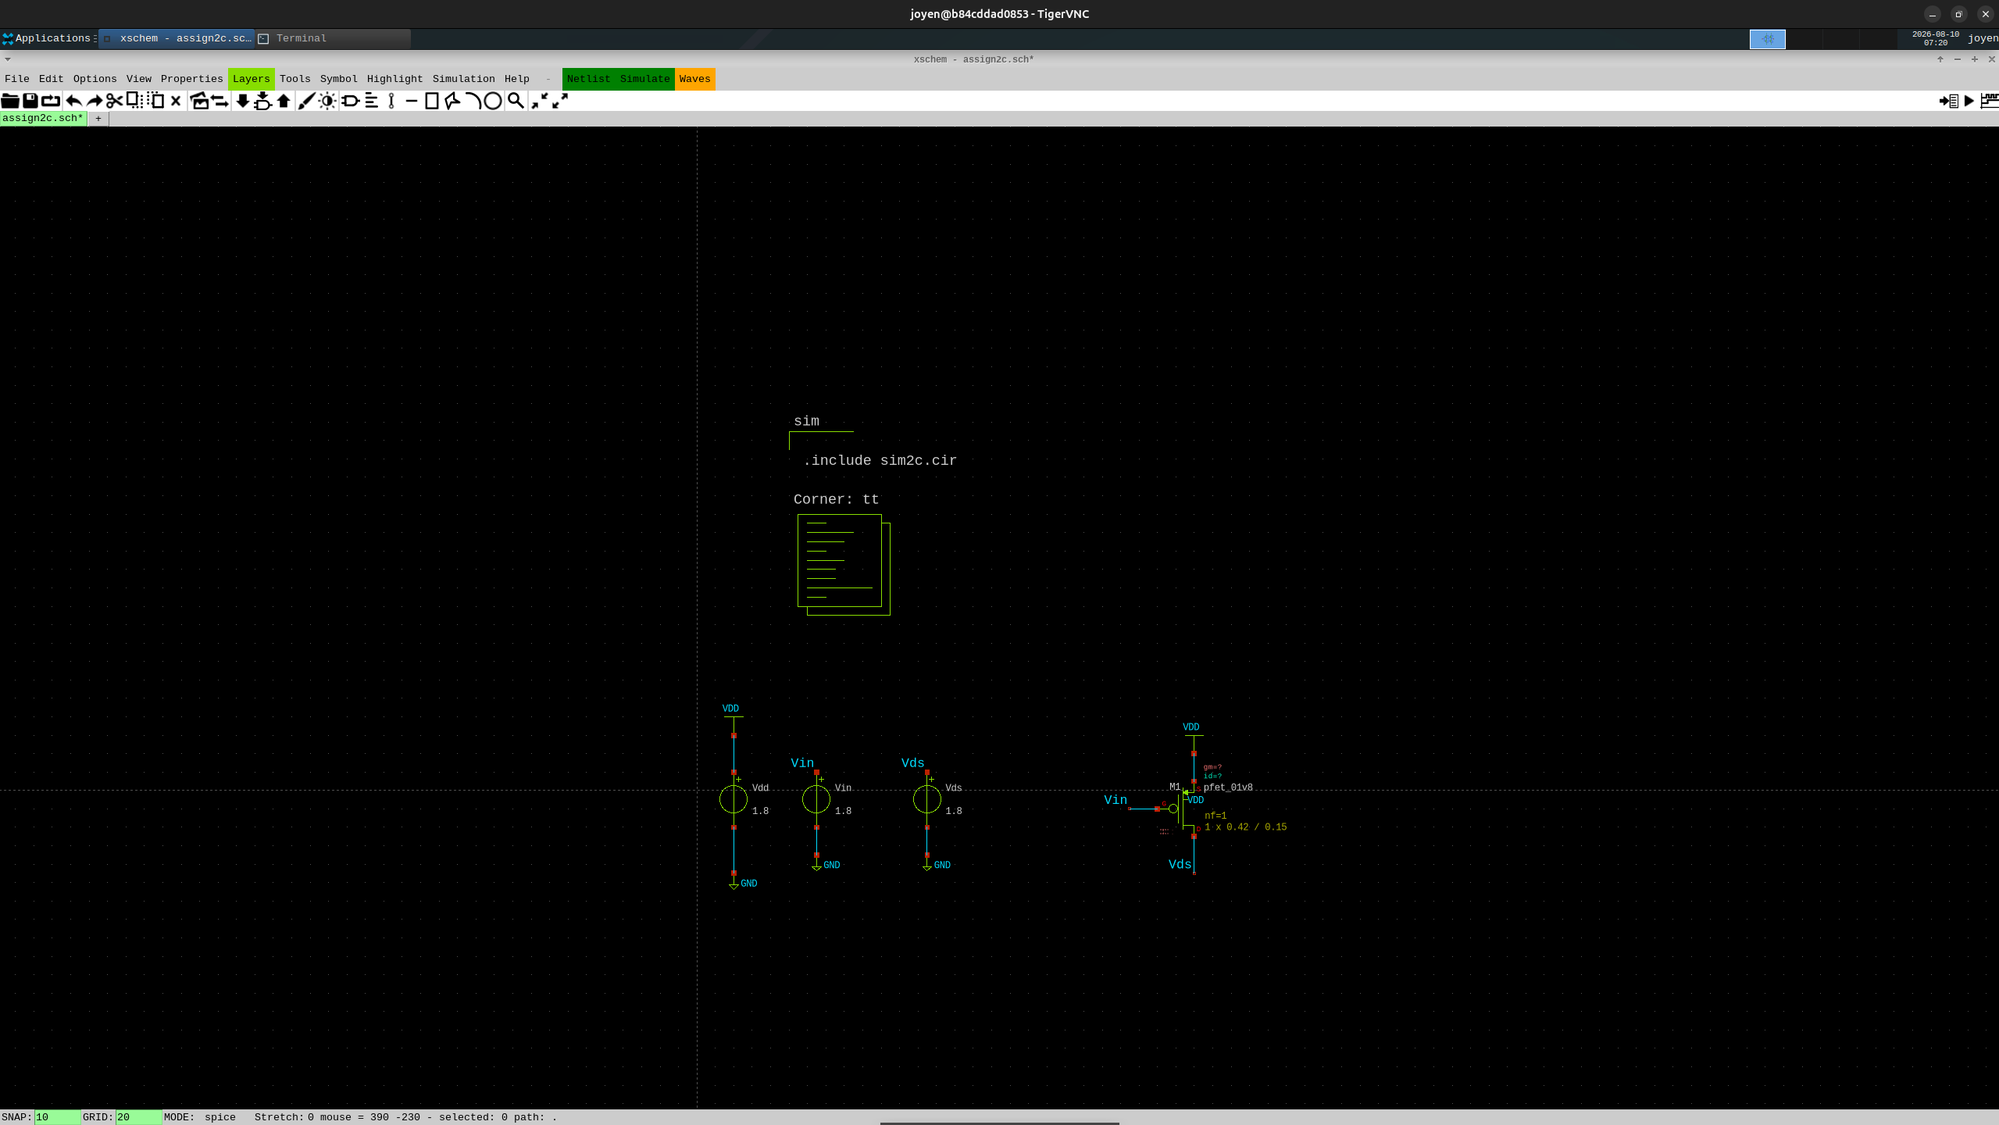
\includegraphics[width=0.8\textwidth]{figures/2c_schematic.png}
  \caption{pMOS with independent gate (\texttt{Vin}, held at 0~V so $V_{sg}=V_{DD}$) and drain (\texttt{Vds}, swept) sources, source/body tied to $V_{DD}$, W/L scaled by \texttt{alterparam} across 10 sizes.}
  \label{fig:2c-schematic}
\end{figure}

\subsubsection{Measurement}

\texttt{sim2c.cir} mirrors \texttt{sim1c.cir}: a \texttt{while} loop over $n=1,\ldots,10$ calls \texttt{alterparam Width/Length}, then \texttt{reset} (required for the parametrized \texttt{W=\{Width\} L=\{Length\}} substitution on \texttt{XM1} to take effect), then re-applies \texttt{alter Vin = 0} (since \texttt{reset} reloads the original netlist and would otherwise restore \texttt{Vin} to its literal default of 1.8~V) before \texttt{run}. $V_{SDSAT,n}$ and $\text{VelSatEffect}_n$ are accumulated into element-indexed vectors and plotted against $L_n$.

\begin{figure}[h]
  \centering
  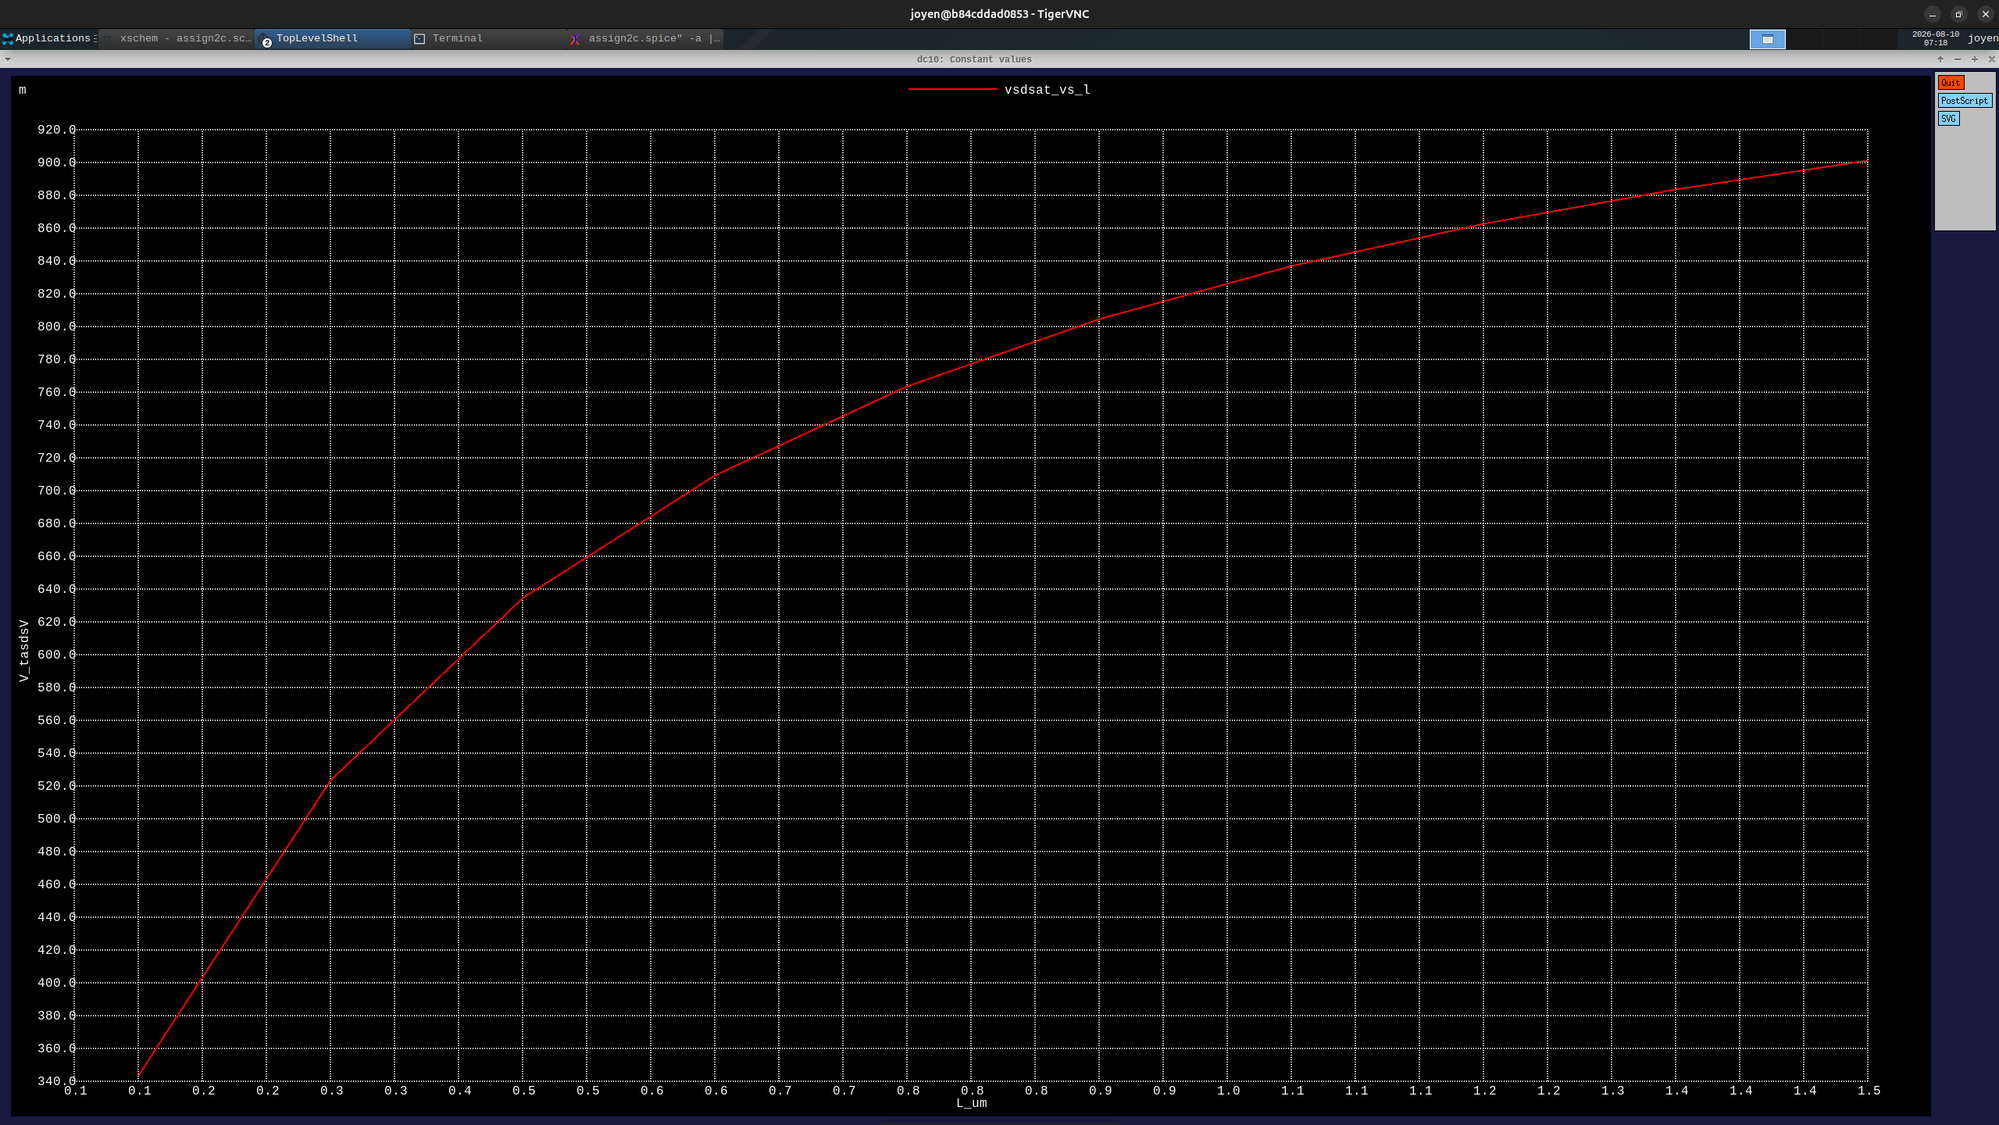
\includegraphics[width=0.8\textwidth]{figures/2c_vsdsat_vs_L.png}
  \caption{Predicted $V_{SDSAT}$ vs.\ channel length $L$: rises from 0.344~V toward the long-channel limit $V_{sgt}=1.1$~V as $L$ grows.}
  \label{fig:2c-vsdsat}
\end{figure}

\begin{figure}[h]
  \centering
  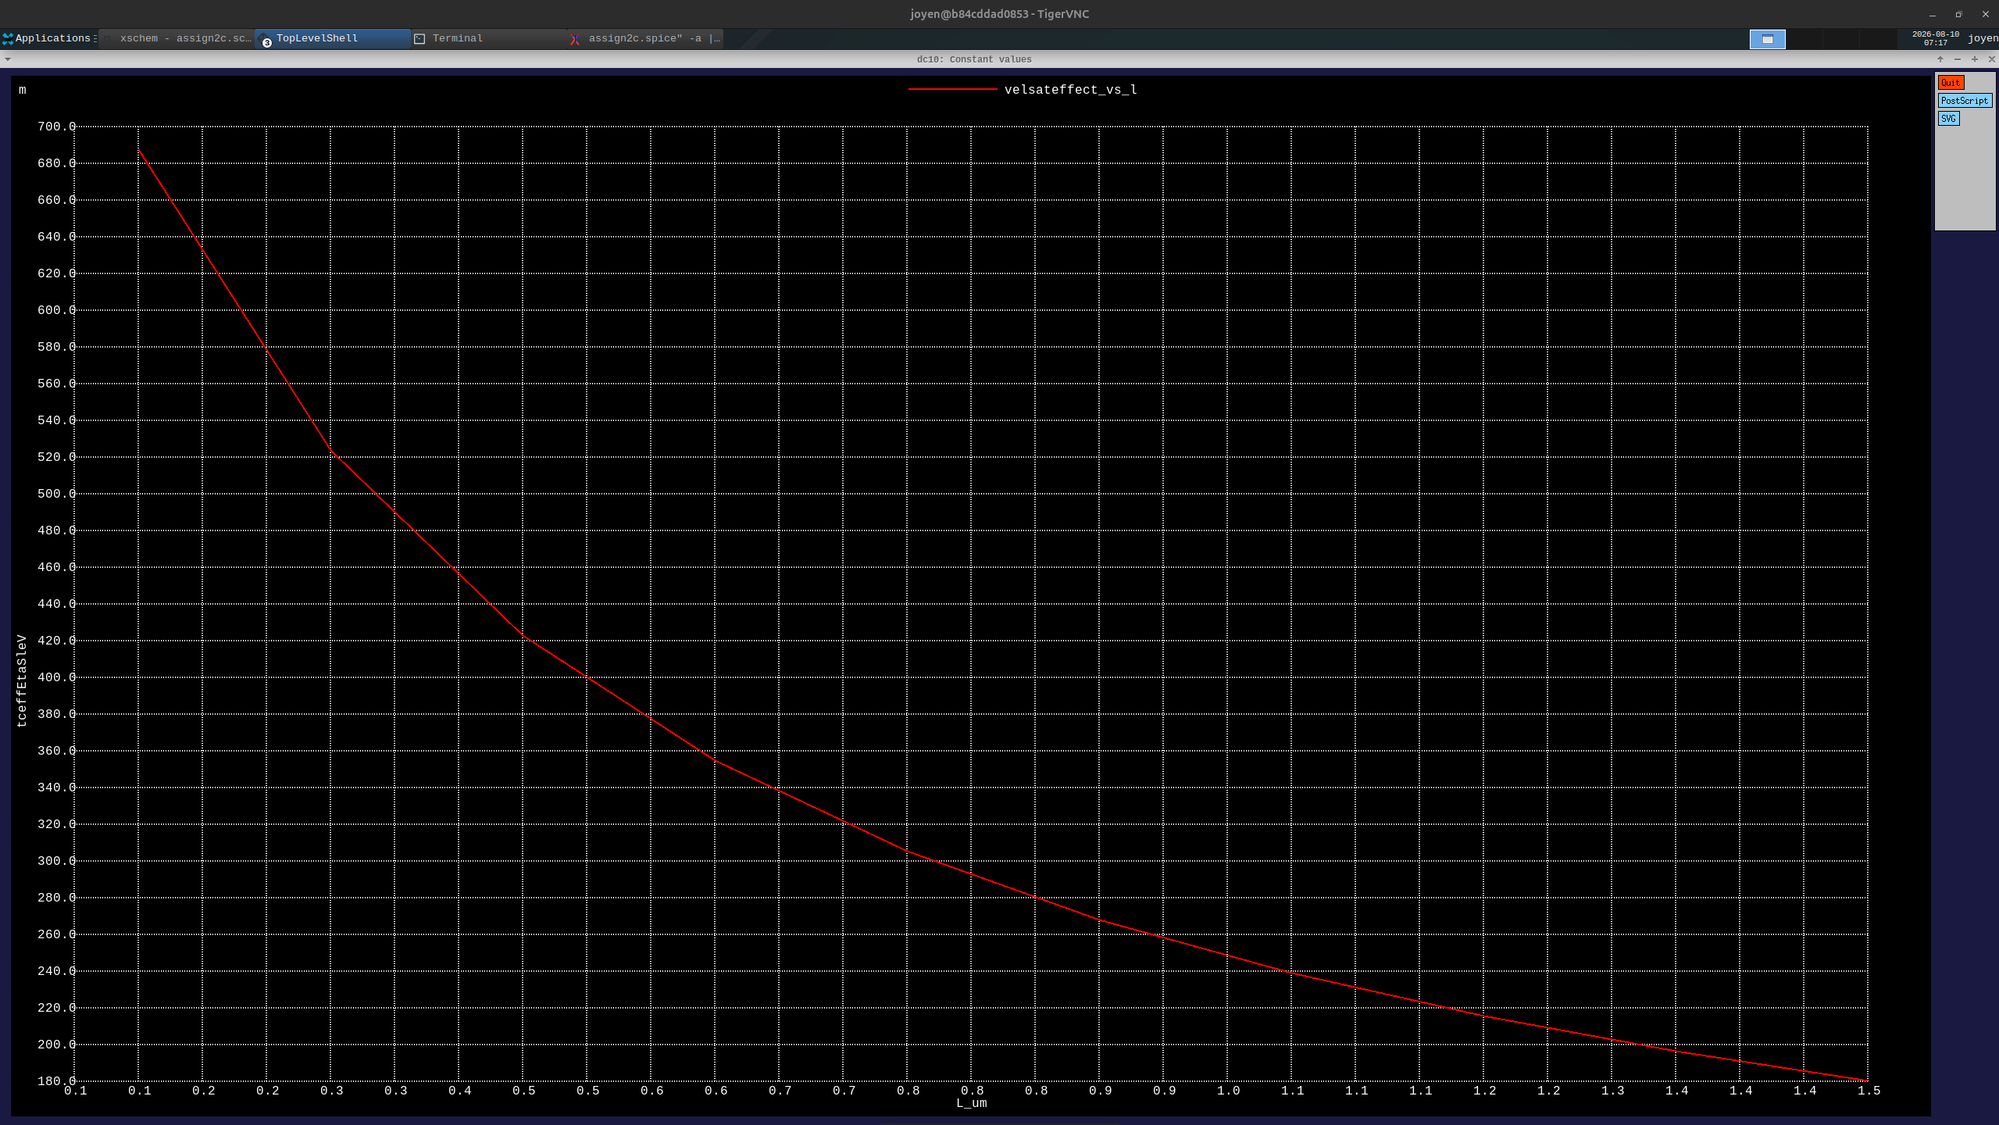
\includegraphics[width=0.8\textwidth]{figures/2c_velsateffect_vs_L.png}
  \caption{Velocity-saturation effect ($1-V_{SDSAT}/V_{sgt}$) vs.\ channel length $L$: decreases monotonically from 0.688 (smallest size) to 0.180 (largest size).}
  \label{fig:2c-velsateffect}
\end{figure}

\paragraph{Discussion.} The pMOS $V_{SDSAT}$ and VelSatEffect curves have exactly the same shape as the nMOS ones from Part 1(c) -- $V_{SDSAT}$ climbing from 0.344~V toward the long-channel value $V_{sgt}=1.1$~V, and VelSatEffect falling monotonically from 0.688 to 0.180, a $3.8\times$ reduction. Comparing directly against Part 1(c)'s nMOS numbers (0.696 at the smallest size, 0.186 at the largest), the pMOS VelSatEffect is slightly \emph{lower} at both ends of the sweep (0.688 vs.\ 0.696; 0.180 vs.\ 0.186) -- a small but consistent gap in the direction predicted by the Calculation above: the pMOS's larger critical field $\xi_{c,p}$ (from its lower hole mobility) gives it a slightly larger $V_{SDSAT}$ for the same $L$, i.e.\ marginally less velocity-saturation compression than the nMOS. The effect is modest for this specific sky130 parameter set ($\xi_{c,p}$ is only $\sim\!4\%$ larger than $\xi_{c,n}$) rather than the dramatic difference Rabaey's generic 0.25~$\mu$m example shows (Figure 3.21, p.~68), but the direction matches exactly what the textbook predicts.

\section{Problem 3}

\subsection{Part (a): nMOS Charging a Capacitor}

Connect a 100fF capacitor to the source terminal of an nMOS ($L=0.15\ \mu\text{m}$, $W=0.42\ \mu\text{m}$), with the drain tied to $V_{DD}=1.8$~V and the gate driven by a step input $V_{in}$ that goes from 0 to $V_{DD}$ at $t=0$ with a 10ps rise time (a PULSE source with a period much longer than the simulation window, so it transitions once and holds). Assuming the capacitor is initially discharged, find $V_{out}$ at $t=20$~ns and $100$~ns, and compare against the analytical $V_{out}(\infty)$.

\subsubsection{Calculation}

This is a source-follower configuration: gate and drain are both eventually at $V_{DD}$, and the source (cap node, $V_{out}$) floats up until the current stops. At steady state $I_{ds}=0$, which requires $V_{gs}=V_{Tn}$ exactly -- independent of which current-vs-voltage model is used:
\[
V_{out}(\infty) = V_{DD} - V_{Tn} = 1.8 - 0.7 = 1.1\ \text{V}
\]
As $V_{out}$ rises, the overdrive $V_{gs}-V_{Tn}$ shrinks, so the charging current (and hence $dV_{out}/dt$) continuously decreases -- this is why the curve rises quickly at first and then flattens asymptotically toward 1.1~V rather than reaching it in finite time.

\subsubsection{Schematic}

\begin{figure}[h]
  \centering
  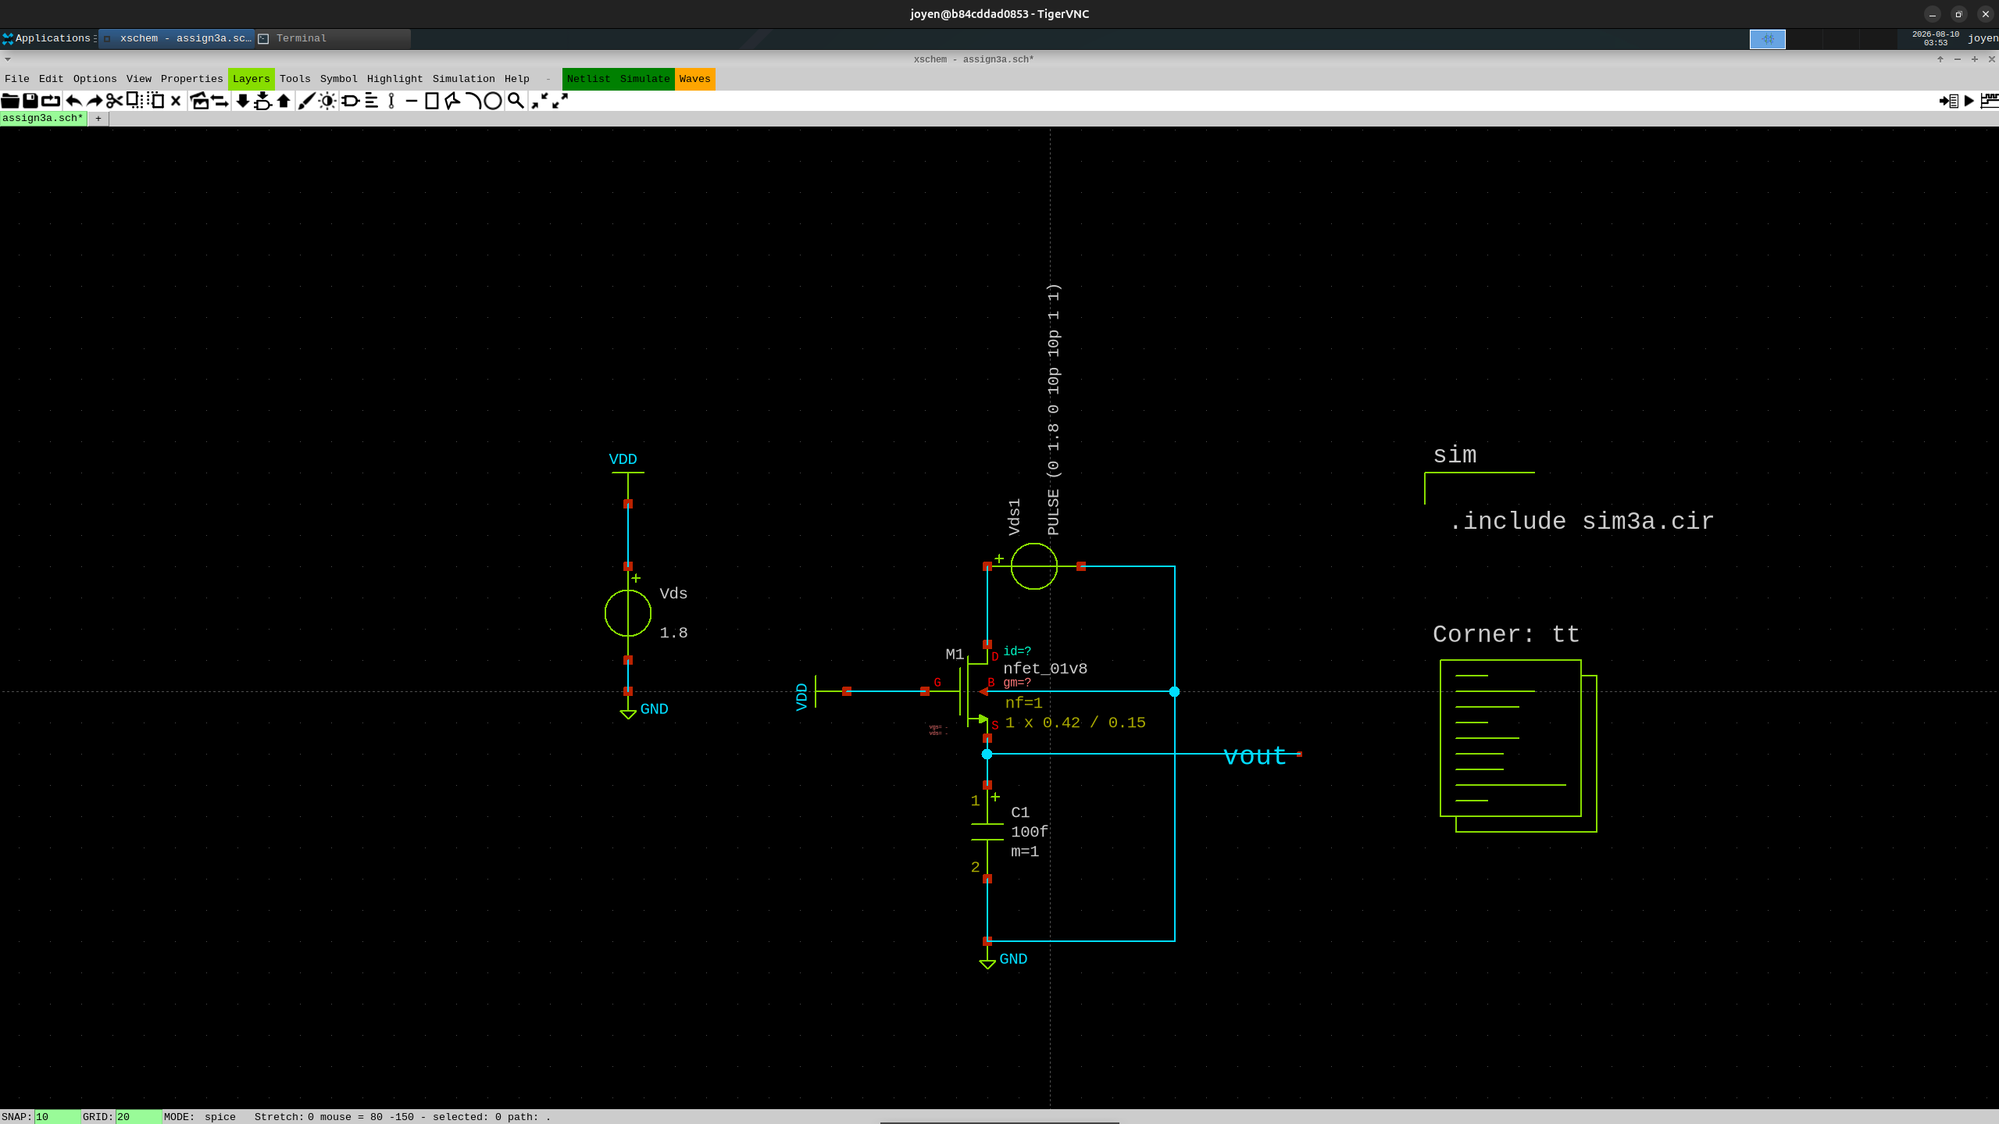
\includegraphics[width=0.8\textwidth]{figures/3a_schematic.png}
  \caption{nMOS with a 100fF capacitor at the source (\texttt{vout}), gate driven by a PULSE step, drain fixed at $V_{DD}$.}
\end{figure}

\subsubsection{Measurement}

\texttt{sim3a.cir} sets \texttt{.ic V(vout)=0}, runs \texttt{tran 1p 150n}, and uses \texttt{meas tran ... find v(vout) at=20n/100n} to extract the two requested values.

\begin{figure}[h]
  \centering
  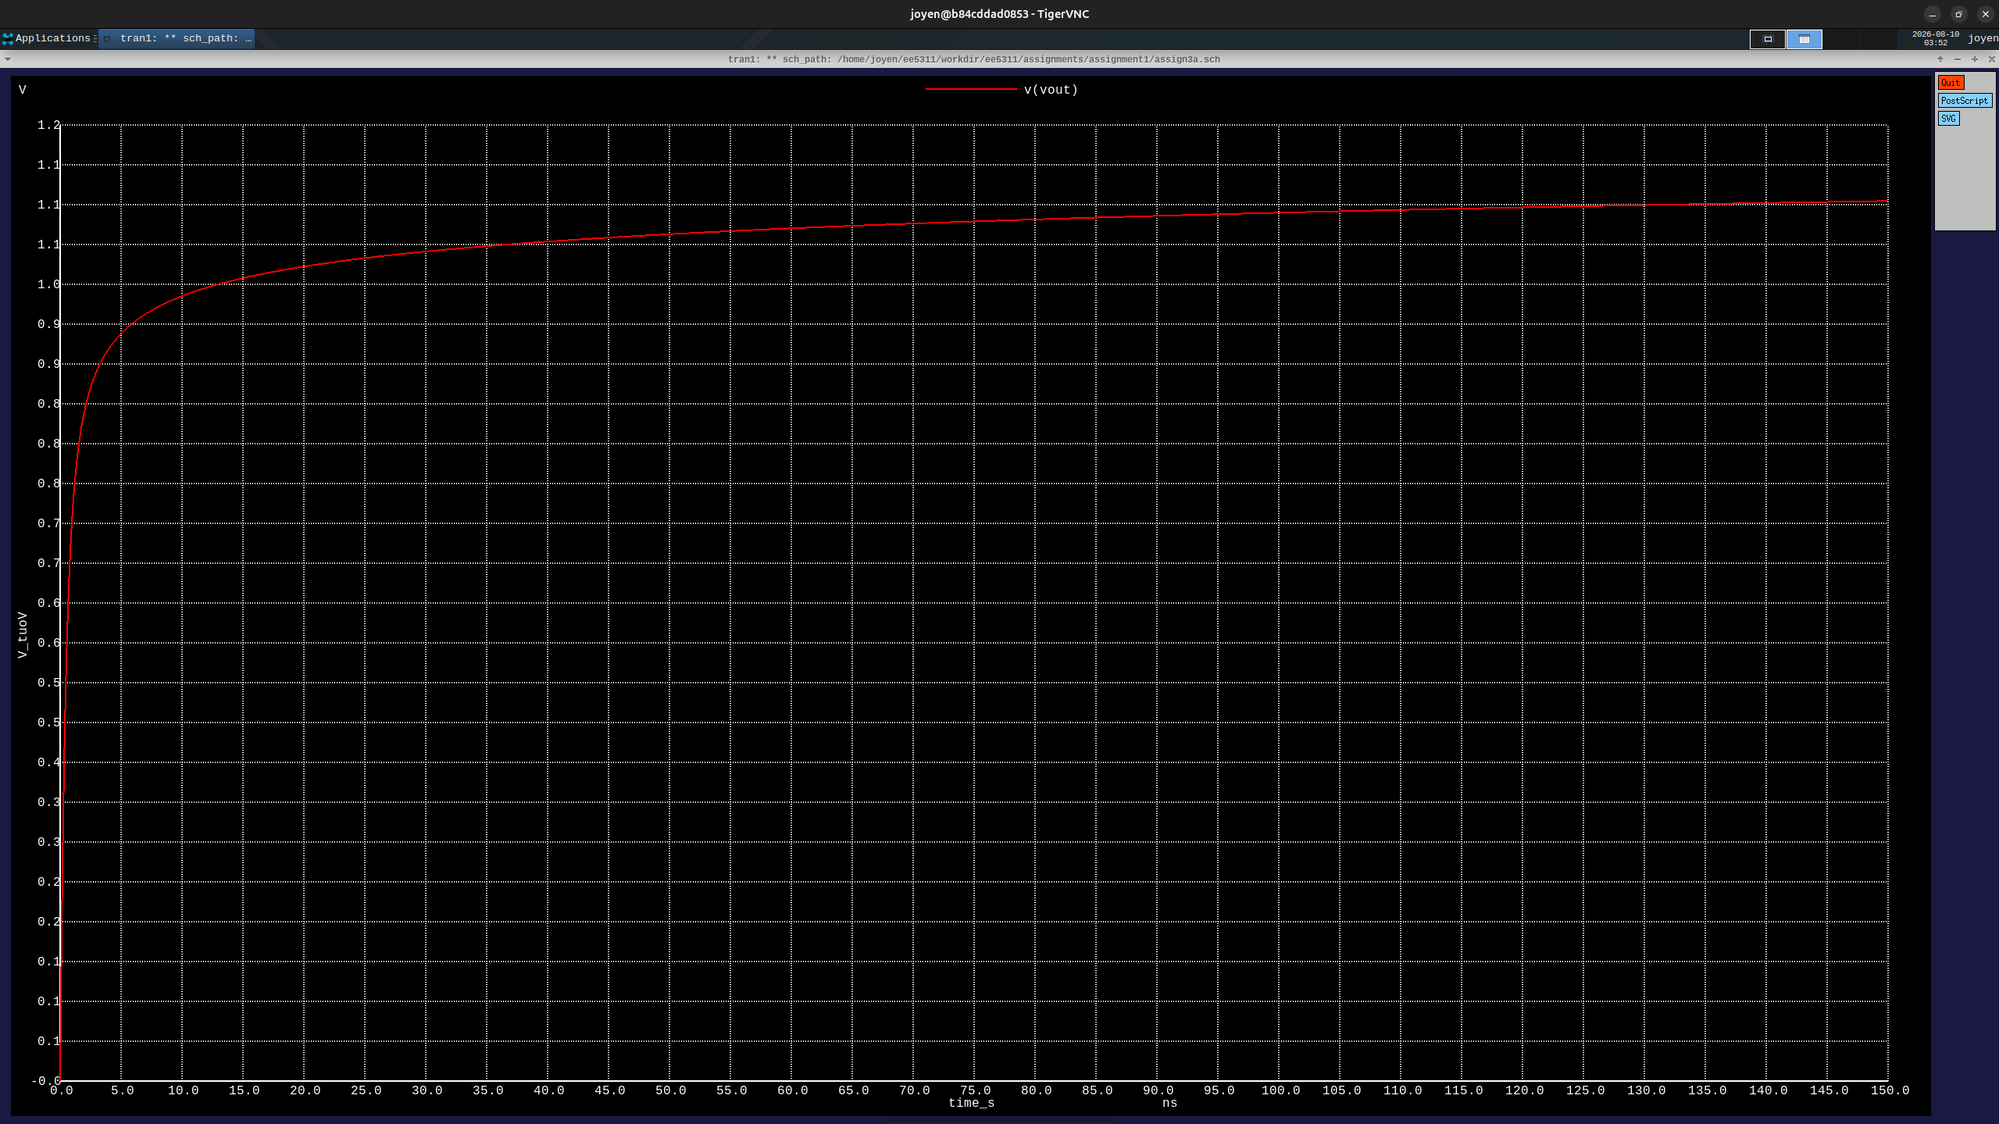
\includegraphics[width=0.95\textwidth]{figures/3a_vout.png}
  \caption{Simulated $V_{out}(t)$: rises quickly, then flattens asymptotically toward the analytical $V_{out}(\infty)=1.1$~V.}
\end{figure}

\paragraph{Effective time constant.} This is not a linear RC circuit -- the charging current depends on $V_{out}$ itself and vanishes as $V_{out}\to V_{DD}-V_{Tn}$ -- so there is no single exponential $\tau$ that describes the whole transient. As an order-of-magnitude estimate, take the saturation current at $t=0^+$ (largest overdrive, $V_{gt}=1.1$~V) using the same Eq.~(3.38)--(3.39) model from Part (a): with $L\xi_c=0.48$~V, $V_{DSAT}=0.334$~V, and $I_{DSAT}\approx\mu_nC_{oxn}\frac{W}{L}(V_{gt}V_{DSAT}-\tfrac12V_{DSAT}^2)\approx182\ \mu\text{A}$. Modeling the transistor as an equivalent resistor $R_{eq}=V_{DSAT}/I_{DSAT}\approx1.84\ \text{k}\Omega$ at this initial operating point gives
\[
\tau \approx R_{eq}C = 1.84\ \text{k}\Omega \times 100\ \text{fF} \approx 184\ \text{ps}, \qquad V_{out,\text{anal}}(t) \approx V_{out}(\infty)\left(1-e^{-t/\tau}\right).
\]

\begin{table}[h]
  \centering
  \begin{tabular}{|c|c|c|}
    \hline
    Quantity & Analytical (RC model) & Simulated \\
    \hline
    $V_{out}(20\text{ns})$  & 1.100 & 1.022 \\
    $V_{out}(100\text{ns})$ & 1.100 & 1.090 \\
    $V_{out}(\infty)$       & 1.100 & -- \\
    \hline
  \end{tabular}
  \caption{Analytical (fixed-$\tau$ RC) prediction vs.\ simulated Vout at 20ns/100ns, and the analytical steady-state value.}
\end{table}

\paragraph{Discussion.} Since $20$~ns and $100$~ns are both $\gg 5\tau\approx920$~ps, the fixed-$\tau$ exponential model predicts $V_{out}$ has already fully settled to $1.100$~V by both time points -- but the simulation shows only $1.022$~V ($93\%$) at 20~ns and $1.090$~V ($99\%$) at 100~ns. The analytical RC estimate is a poor match at both points, and increasingly so at early times: it assumes a constant conductance $1/R_{eq}$ set by the $t=0^+$ overdrive, but the real conductance (and hence the charging current) drops continuously as $V_{out}$ rises toward $V_{DD}-V_{Tn}$, so the true response decays far slower than a fixed-$\tau$ exponential -- the effective $\tau$ grows without bound as $V_{out}\to V_{DD}-V_{Tn}$. This is the expected signature of the nonlinear, self-limiting source-follower charging behavior, not a modeling error.

\subsection{Part (b): pMOS Drain Node Driven by an Ideal Source}

Same 100fF capacitor and pMOS device size, this time with the pMOS gate held fixed at GND and source/body tied to $V_{DD}=1.8$~V (so $V_{sg}=1.8$~V, $M1$ is always fully on), and a step applied directly to the drain node, which also carries the capacitor.

\subsubsection{Calculation}

This circuit is structurally different from Part (a)/(c) in one important respect: the capacitor $C1$ and the independent source driving the step are wired to the \emph{same} node (the drain). An ideal voltage source unconditionally pins the voltage at the node it is connected to, regardless of any current flowing into or out of that node from elsewhere (here, from $M1$'s channel). Consequently:
\[
V_{ds}(t) = V_{\text{PULSE}}(t) \qquad \text{exactly, for all } t,
\]
i.e.\ $V_{ds}(t)$ is simply the applied PULSE waveform itself -- a linear ramp from $1.8$~V to $0$~V over the specified $10$~ps fall time, then flat at $0$~V. There is no RC-style exponential governed by $M1$'s channel resistance here, unlike Parts (a)/(c): $M1$'s conduction state is irrelevant to $V_{ds}(t)$, because the ideal source's zero output impedance overwhelms whatever current the transistor tries to source or sink. The capacitor's presence does not change this curve at all -- the same $V_{ds}(t)$ would result with $C1$ removed entirely. This is the key qualitative contrast with Parts (a)/(c), where the capacitor was the \emph{only} thing on its node (no competing ideal source), so the transistor's channel resistance was what actually set the timescale of the transient.

\subsubsection{Schematic}

\begin{figure}[h]
  \centering
  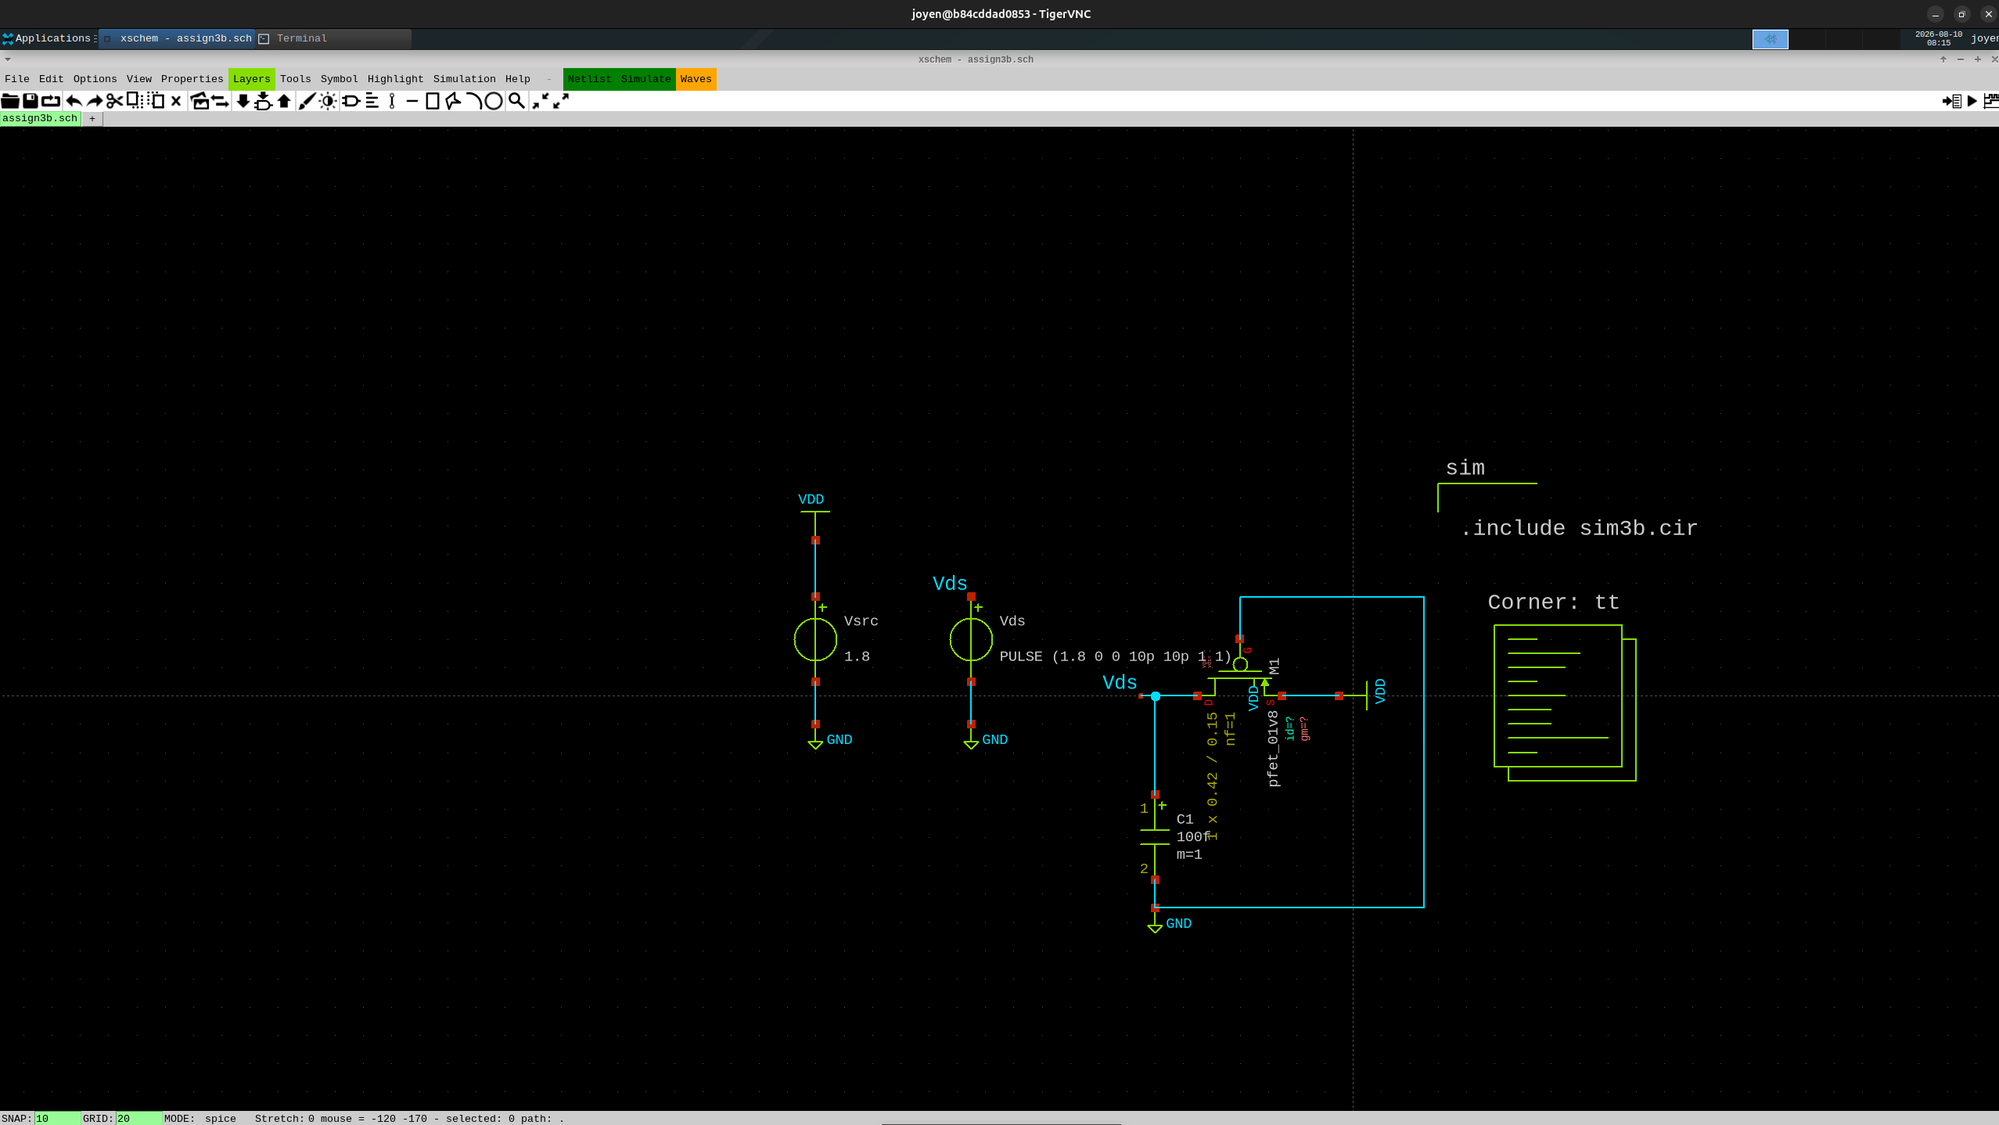
\includegraphics[width=0.9\textwidth]{figures/3b_schematic.png}
  \caption{pMOS with gate fixed at GND, source/body fixed at $V_{DD}$, and the PULSE source \texttt{Vds} wired to the same node as the drain and the capacitor $C1$.}
  \label{fig:3b-schematic}
\end{figure}

\subsubsection{Measurement}

\texttt{sim3b.cir} runs \texttt{tran 1p 150n} with \texttt{.ic V(vds)=1.8}, and measures $V_{ds}$ at $20$~ns and $100$~ns:

\begin{verbatim}
.ic V(vds)=1.8
.control
  tran 1p 150n
  let vt_p = 0.7
  meas tran vds_20ns  find v(vds) at=20n
  meas tran vds_100ns find v(vds) at=100n
  plot v(vds) xlabel time_s ylabel Vds_V
  plot i(Vsrc) xlabel time_s ylabel I_Vsrc_A
  plot v(vds) xlimit 0 200p xlabel time_s ylabel Vds_V
.endc
\end{verbatim}

\begin{figure}[h]
  \centering
  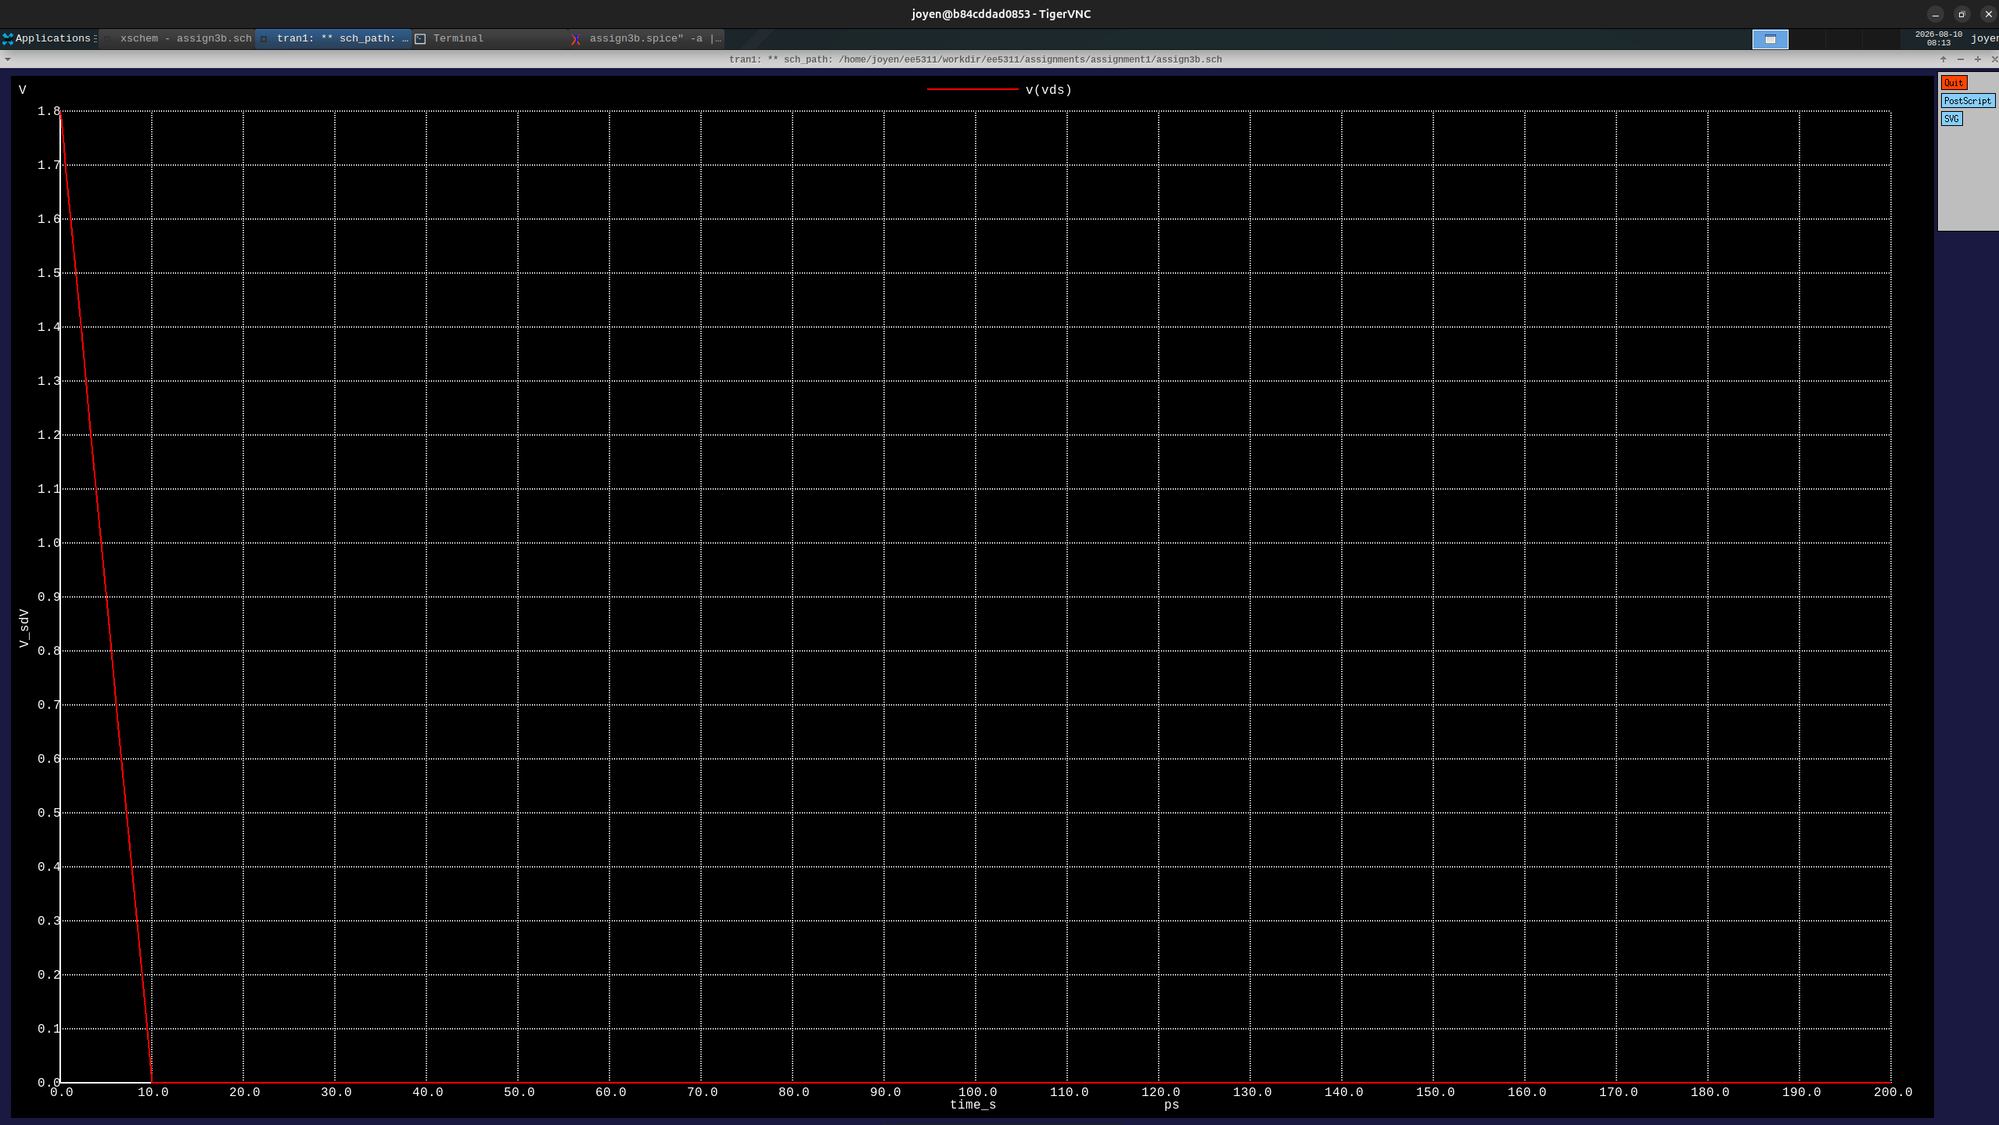
\includegraphics[width=0.95\textwidth]{figures/3b_vds_zoom.png}
  \caption{Simulated $V_{ds}(t)$, zoomed to the first 200ps: a linear fall from 1.8~V to 0~V over the PULSE's 10ps fall time, then flat at 0~V -- exactly reproducing the applied waveform.}
  \label{fig:3b-measurement}
\end{figure}

\begin{table}[h]
  \centering
  \begin{tabular}{|c|c|c|}
    \hline
    Quantity & Applied waveform (exact) & Simulated \\
    \hline
    $V_{ds}(20\text{ns})$  & 0 & 0.000 \\
    $V_{ds}(100\text{ns})$ & 0 & 0.000 \\
    \hline
  \end{tabular}
  \caption{$V_{ds}$ at 20ns/100ns: both the applied waveform and the simulated result are exactly 0~V (to the precision ngspice printed), $\sim\!2000\times$ past the 10ps fall time.}
  \label{tab:3b-error}
\end{table}

\paragraph{Discussion.} Unlike Part (a) (where the fixed-$\tau$ RC estimate was only an \emph{approximation} of the real, nonlinear source-follower transient, and disagreed with simulation by tens of percent), here there is nothing to approximate: the ``analytical model'' for $V_{ds}(t)$ is just the literal PULSE waveform written into the netlist, so simulated and applied agree to within solver precision by construction -- an exact match is not evidence that the transistor's physics was captured correctly, it just confirms the ideal source is doing exactly what an ideal source does. The genuinely useful signal in this circuit is $i(V_{src})$ (the current drawn from the fixed $V_{DD}$ supply through $M1$'s source/body), which does reflect $M1$ actually conducting during the transition. The broader lesson from contrasting Part (b) against Parts (a)/(c): whether a transistor's channel resistance actually sets an RC timescale, or is rendered irrelevant by a stiffer ideal source sharing the same node, depends entirely on the topology -- the capacitor must be on a node with no competing low-impedance driver for its charge/discharge behavior to reveal anything about the device.

\subsection{Part (c): nMOS Discharging a Capacitor}

Same nMOS and 100fF capacitor at the source node (\texttt{vout}), but now the gate is held fixed at $V_{DD}=1.8$~V for the entire simulation, and the step is applied to the drain instead: a PULSE source takes the drain from $V_{DD}$ down to $0$~V at $t=0$ with a 10ps fall time. The capacitor starts fully charged, $V_{out}(0)=1.8$~V. Find $V_{out}$ at $t=20$~ns and $100$~ns.

\subsubsection{Calculation}

Once the drain is pulled to $0$~V, it becomes the lower-voltage terminal, so it takes over as the MOSFET's physical source for as long as $V_{out}>0$. The gate is fixed at $V_{DD}$ throughout, so the overdrive seen by the device is
\[
V_{gt} = V_{DD} - V_{Tn} = 1.8 - 0.7 = 1.1\ \text{V},
\]
constant for the whole transient -- unlike Part (a), where the overdrive shrank as $V_{out}$ rose and self-limited the charging current. Here nothing shrinks it, so the discharge keeps going all the way to
\[
V_{out}(\infty) = 0\ \text{V},
\]
with no threshold-drop penalty. This is the textbook asymmetry between nMOS pull-up (stops at $V_{DD}-V_{Tn}$) and nMOS pull-down (reaches all the way to $0$): the same device that could only weakly pull $V_{out}$ up to $1.1$~V in Part (a) pulls it fully down to $0$~V here, because the terminal that ends up acting as the source is different in the two cases.

Using the same Eq.~(3.37)--(3.39) model and the same operating point as Part (a) ($V_{gt}=1.1$~V $\Rightarrow V_{DSAT}=0.334$~V, $I_{DSAT}\approx182\ \mu\text{A}$, $R_{eq}=V_{DSAT}/I_{DSAT}\approx1.84\ \text{k}\Omega$), the discharge is well approximated in two phases, since $V_{gt}$ is fixed for the whole transient rather than just at $t=0^+$:
\begin{itemize}
  \item \textbf{Saturation phase} ($V_{out}>V_{DSAT}$): the device stays saturated at essentially constant current $I_{DSAT}$, so $V_{out}$ ramps down \emph{linearly}, not exponentially: $\Delta t_1 = C\,(1.8-V_{DSAT})/I_{DSAT} \approx 100\text{fF}\times1.466\text{V}/182\ \mu\text{A}\approx806\ \text{ps}$.
  \item \textbf{Triode phase} ($V_{out}<V_{DSAT}$): the device behaves as a resistor $R_{eq}$, giving a genuine exponential tail $V_{out}(t)\approx V_{DSAT}\,e^{-t/\tau}$ with $\tau\approx R_{eq}C\approx184$~ps.
\end{itemize}
Both phases together bring $V_{out}$ to within numerical noise of $0$~V by roughly $806\ \text{ps} + 5\tau \approx 1.7$~ns -- more than four orders of magnitude before the first measurement point at $20$~ns.

\subsubsection{Schematic}

\begin{figure}[h]
  \centering
  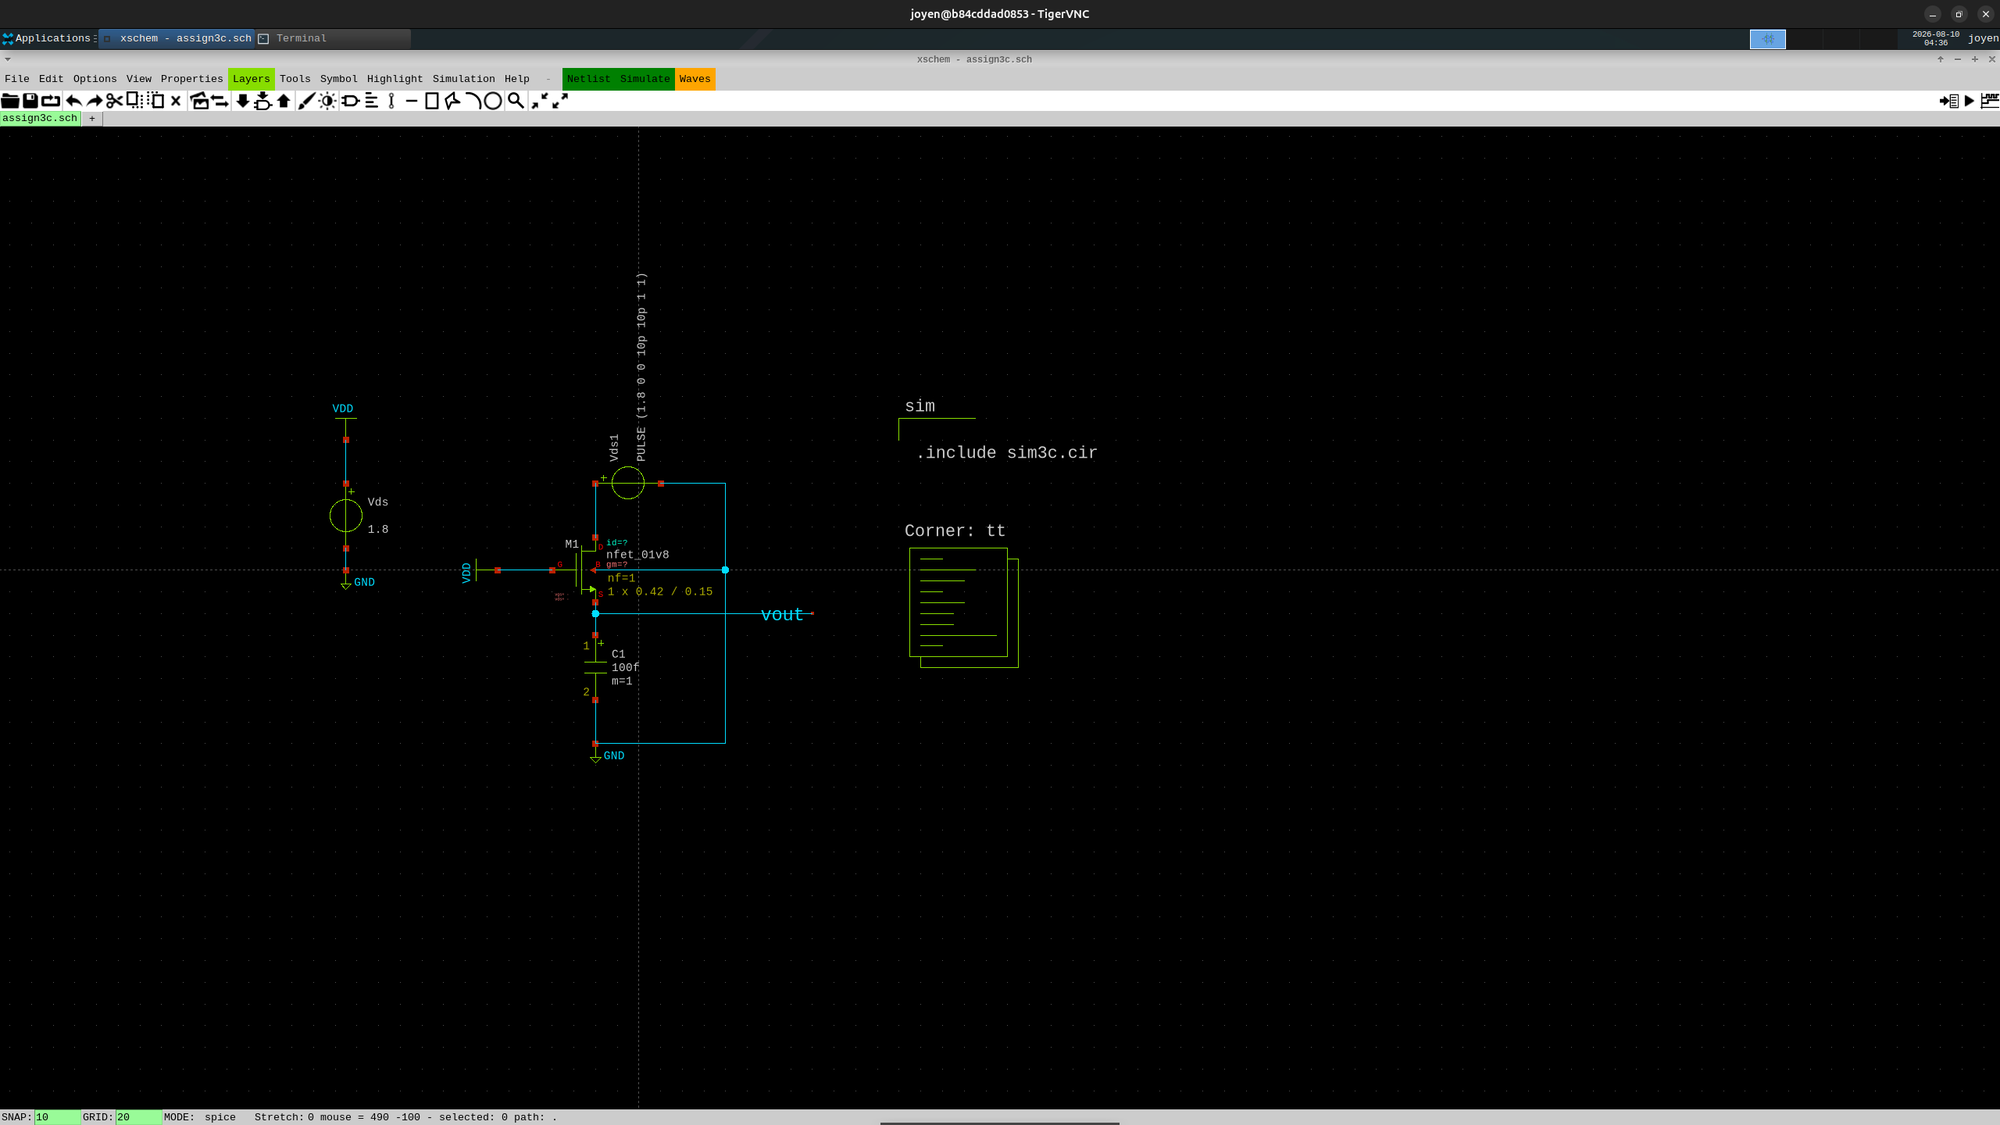
\includegraphics[width=0.8\textwidth]{figures/3c_schematic.png}
  \caption{Same nMOS/capacitor pair as Part (a); the gate is now tied to a fixed $V_{DD}$ source, and the PULSE source drives the drain from $V_{DD}$ to $0$.}
\end{figure}

\subsubsection{Measurement}

\texttt{sim3c.cir} sets \texttt{.ic V(vout)=1.8}, runs \texttt{tran 1p 150n}, and measures $V_{out}$ at $20$~ns and $100$~ns.

\begin{figure}[h]
  \centering
  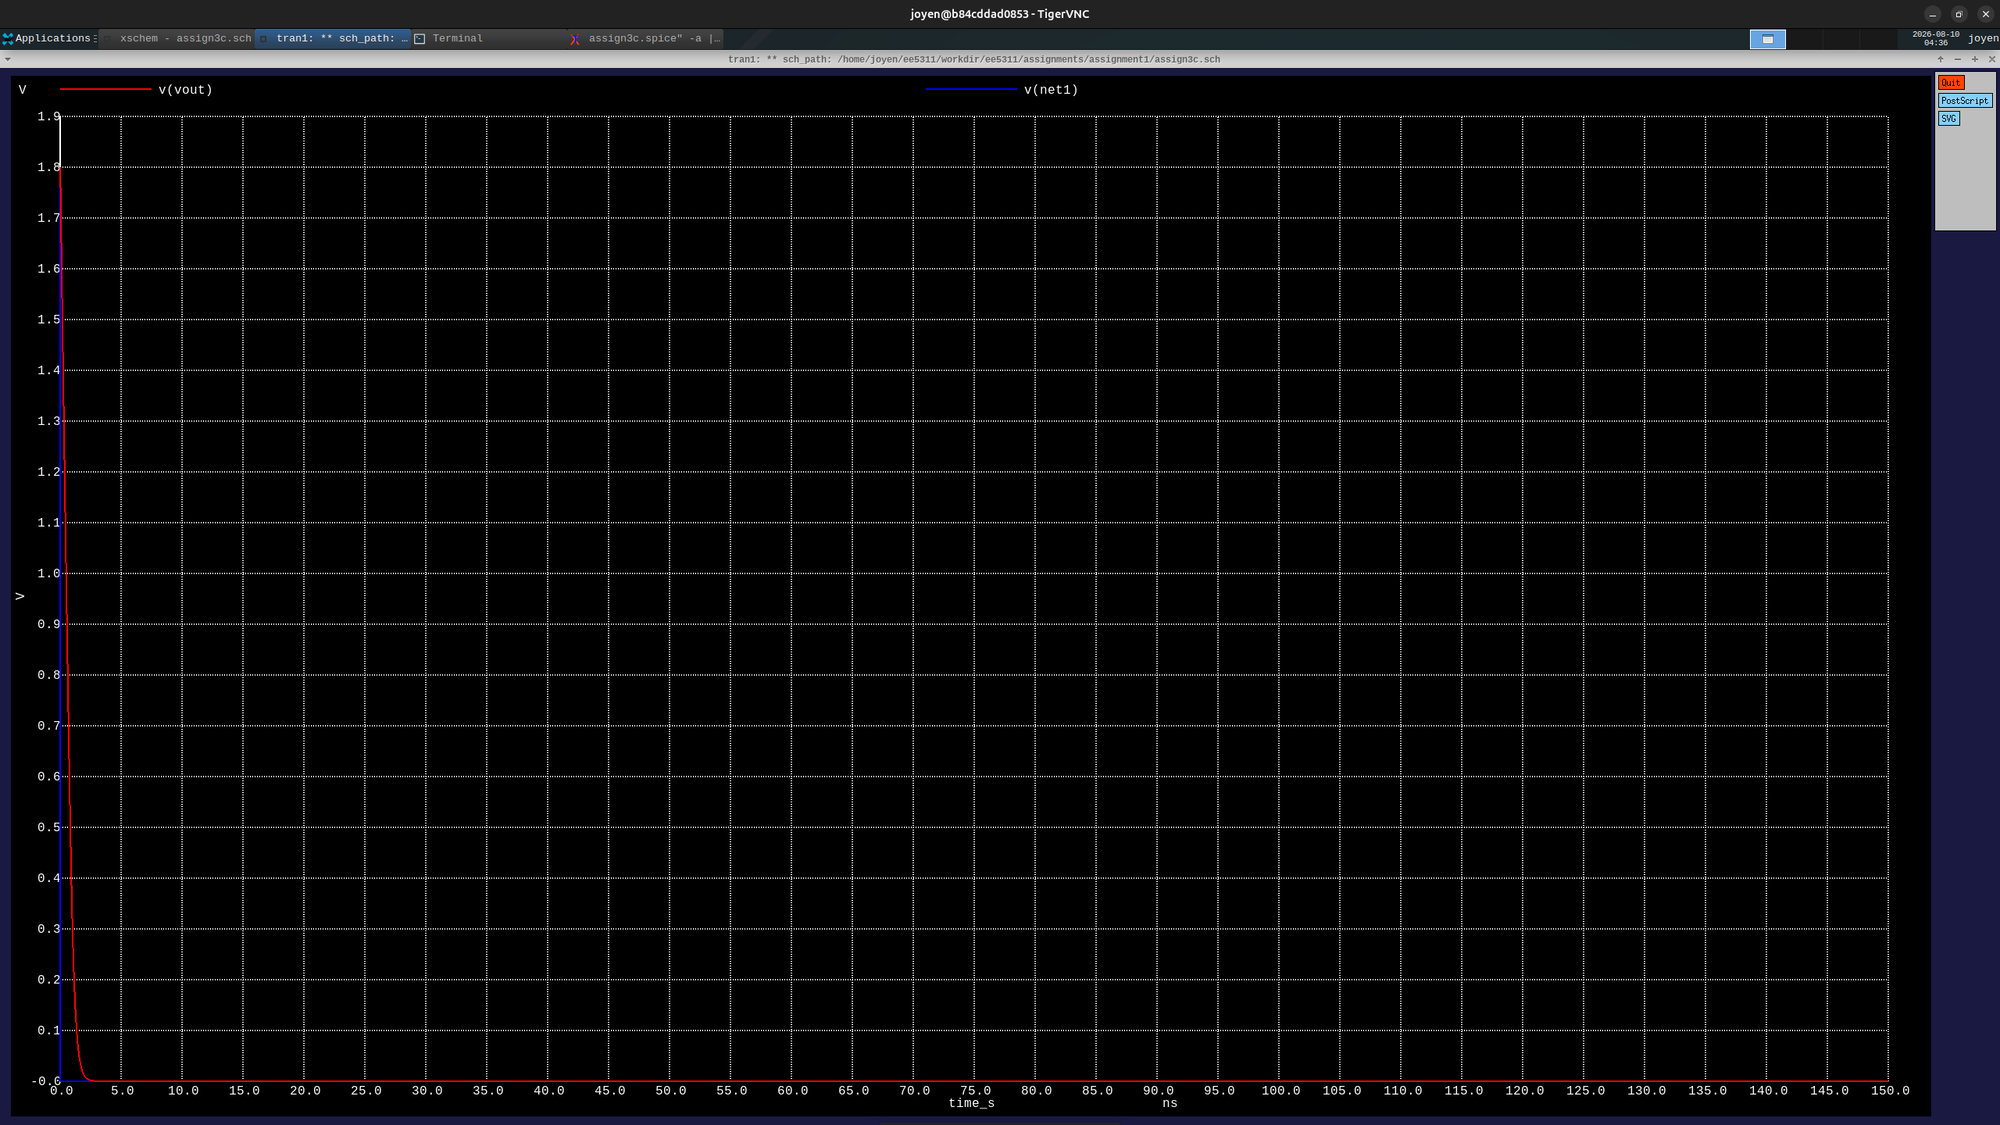
\includegraphics[width=0.95\textwidth]{figures/3c_vout.png}
  \caption{Simulated $V_{out}(t)$ and $V(\text{net1})$: both collapse from $1.8$~V to $\approx0$~V within about a nanosecond and stay there.}
\end{figure}

\begin{table}[h]
  \centering
  \begin{tabular}{|c|c|c|}
    \hline
    Quantity & Analytical (two-phase RC model) & Simulated \\
    \hline
    $V_{out}(20\text{ns})$  & $\approx0$ & $-5.3\times10^{-16}$ \\
    $V_{out}(100\text{ns})$ & $\approx0$ & $-5.4\times10^{-16}$ \\
    $V_{out}(\infty)$       & $0$        & -- \\
    \hline
  \end{tabular}
  \caption{Analytical two-phase (linear then RC) prediction vs.\ simulated Vout at 20ns/100ns, and the analytical steady-state value. Simulated values are at the solver's numerical noise floor, i.e.\ indistinguishable from exactly $0$~V.}
\end{table}

\paragraph{Discussion.} Unlike Part (a), where the fixed-$\tau$ model disagreed with the simulation because the real charging current kept shrinking, here the two-phase model and the simulation agree closely: since the gate overdrive never shrinks (the gate never moves), the device discharges the capacitor essentially as fast as this simple model predicts, reaching $0$~V well within a couple of nanoseconds. The practical takeaway is the classic nMOS pull-up/pull-down asymmetry -- an nMOS can pull a node fully down to $0$~V (no $V_{Tn}$ penalty) but can only pull it up to $V_{DD}-V_{Tn}$ -- and it also illustrates why the \emph{same} physical circuit (nMOS + capacitor at the source) can look wildly different depending on which terminal actually switches: in Part (a) the switching terminal ended up degrading the drive strength as $V_{out}$ approached its target, while here it does not, because the terminal that becomes the effective source ($0$~V, fixed) never moves.

\subsection{Part (d): pMOS Capacitor Across the Supply Rails}

Same pMOS bias as Part (b) (gate fixed at GND, source/body fixed at $V_{DD}$, drain pulsed via the same PULSE waveform), but this time the 100fF capacitor $C1$ is connected directly across $V_{DD}$ and GND instead of sharing a node with the pulsed drain.

\subsubsection{Calculation}

This is an even more extreme version of Part (b)'s caveat. The resolved netlist is
\[
\texttt{XM1 Vds GND VDD VDD ...} \qquad \texttt{Vsrc VDD GND 1.8} \qquad \texttt{C1 VDD GND 100f}
\]
so $C1$ sits on the $V_{DD}$ node, which is \emph{already} pinned by the ideal source \texttt{Vsrc} -- and, unlike Part (b), $C1$ does not even share a node with $M1$'s pulsed drain. There is consequently no node in this circuit where $M1$'s conduction state, or the capacitor, can influence anything: $V_{DD}$ is fixed at $1.8$~V by \texttt{Vsrc} regardless of $C1$, and $V_{ds}$ (the drain node) is fixed by the \texttt{Vds} PULSE source regardless of $M1$ or $C1$. The predicted result is that $V(V_{DD})$ stays flat at exactly $1.8$~V for the entire transient -- not because the pMOS successfully holds the node there against some discharge attempt, but because nothing in this topology ever asks it to move.

\subsubsection{Schematic}

\begin{figure}[h]
  \centering
  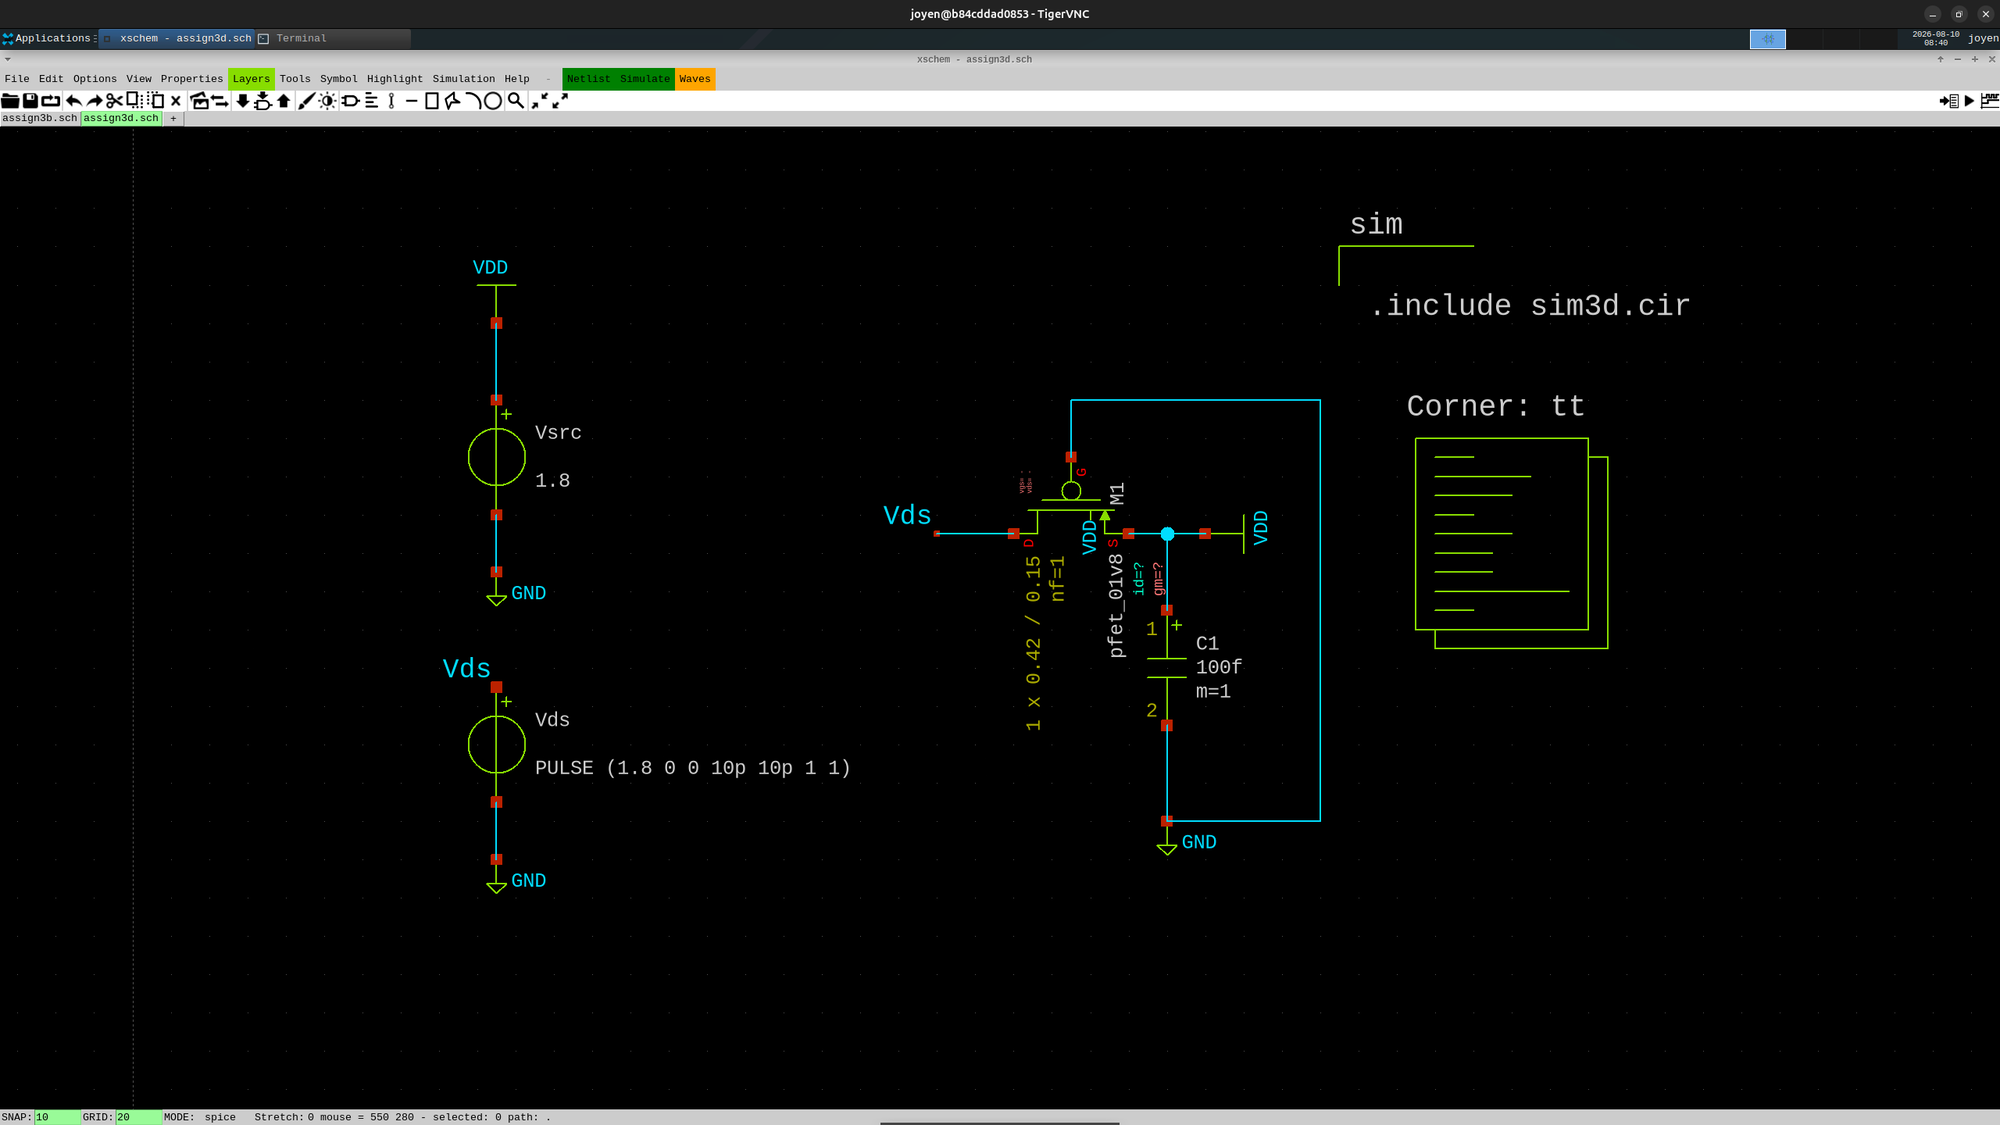
\includegraphics[width=0.9\textwidth]{figures/3d_schematic.png}
  \caption{Same $M1$ bias as Part (b); $C1$ now sits directly on the $V_{DD}$ node (visible junction dot between $M1$'s source pin, the $V_{DD}$ label, and $C1$'s top plate), sharing no node with the pulsed drain.}
  \label{fig:3d-schematic}
\end{figure}

\subsubsection{Measurement}

\texttt{sim3d.cir} runs the same \texttt{tran 1p 150n} as Part (b), additionally measuring $V(V_{DD})$ to make the capacitor's disconnection directly visible in the results:

\begin{verbatim}
.ic V(vds)=1.8
.control
  tran 1p 150n
  let vt_p = 0.7
  meas tran vds_20ns  find v(vds) at=20n
  meas tran vds_100ns find v(vds) at=100n
  meas tran vdd_20ns  find v(vdd) at=20n
  meas tran vdd_100ns find v(vdd) at=100n
  plot v(vds) xlabel time_s ylabel Vds_V
  plot v(vdd) xlabel time_s ylabel Vdd_V
  plot i(Vsrc) xlabel time_s ylabel I_Vsrc_A
  plot v(vds) xlimit 0 200p xlabel time_s ylabel Vds_V
.endc
\end{verbatim}

\begin{figure}[h]
  \centering
  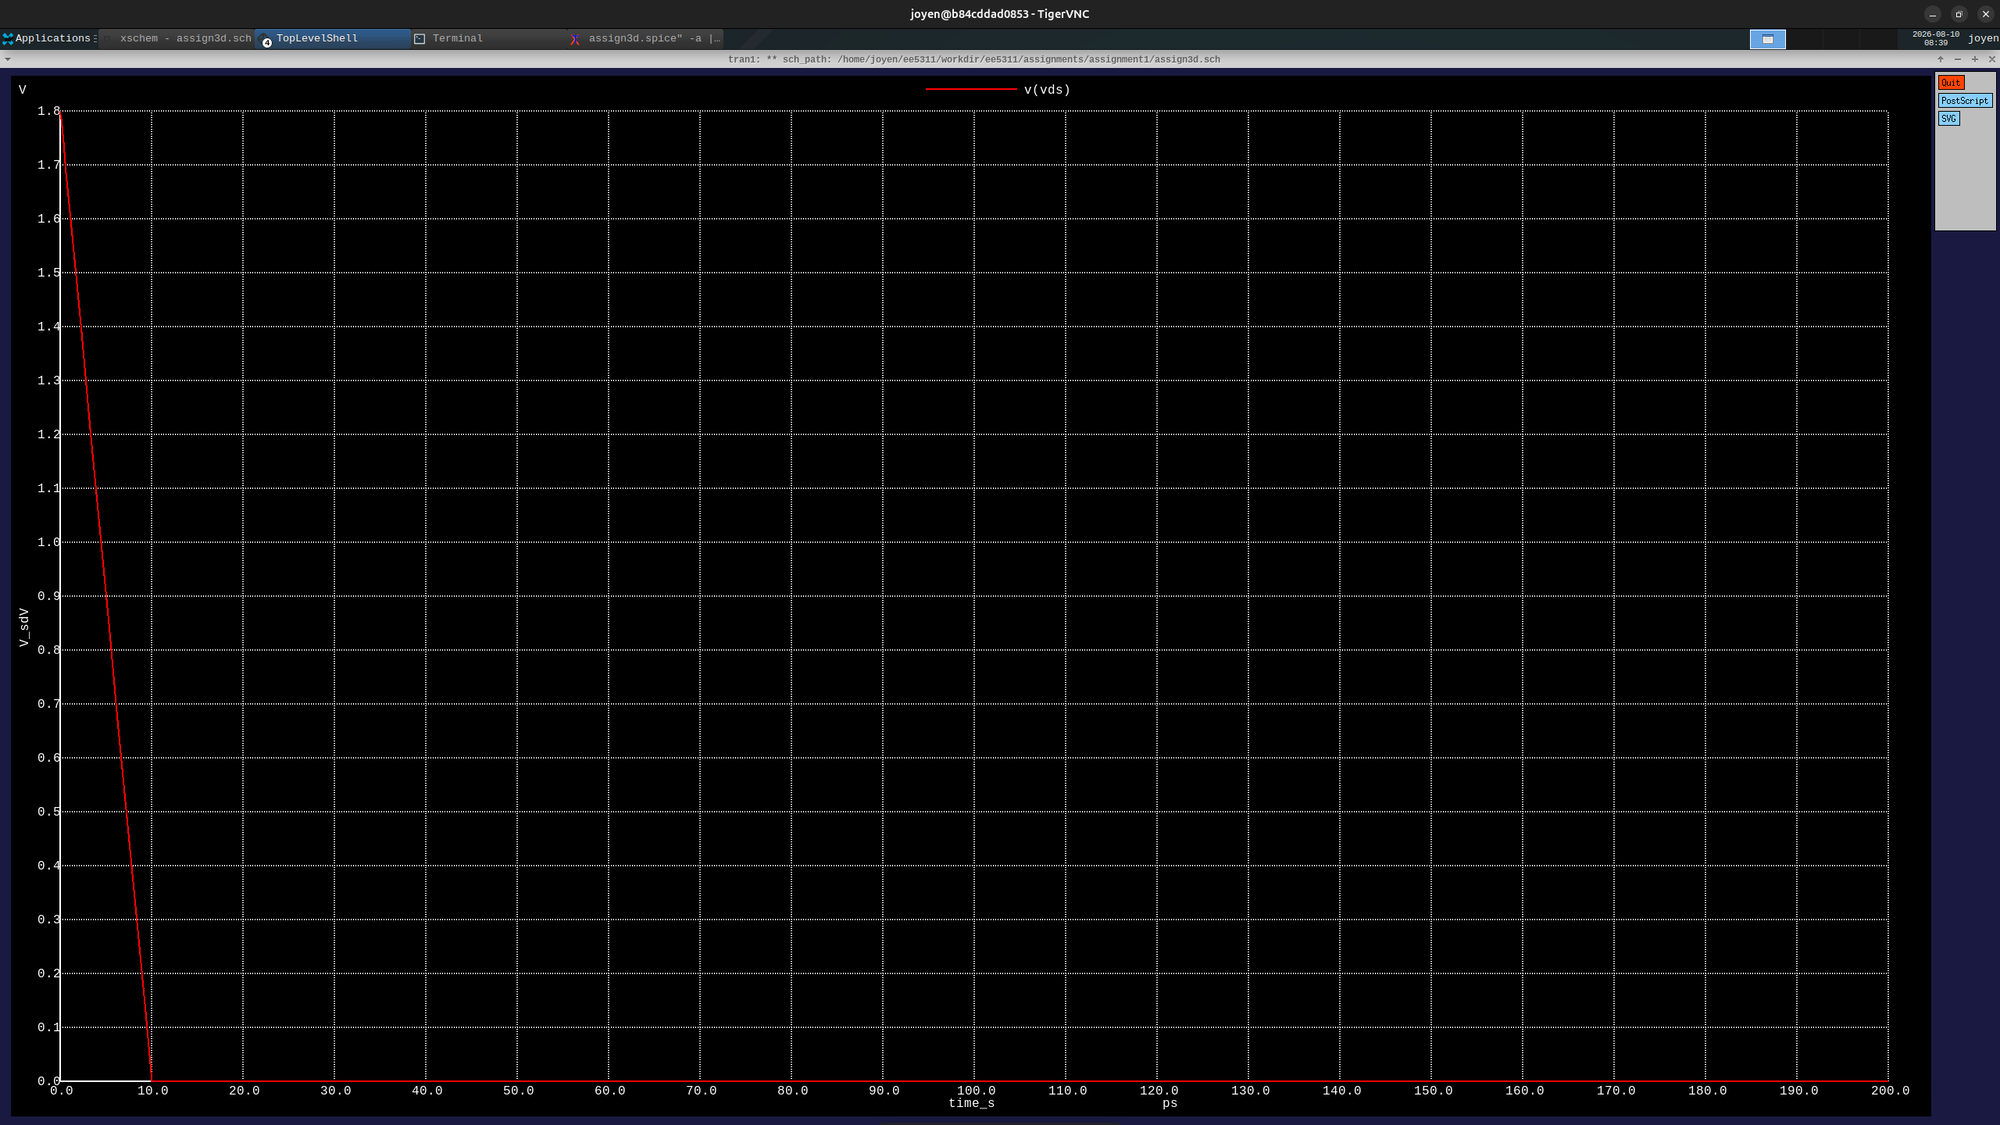
\includegraphics[width=0.95\textwidth]{figures/3d_vds_zoom.png}
  \caption{Simulated $V_{ds}(t)$, zoomed to the first 200ps: identical in shape to Part (b)'s, since $M1$'s drain bias is unchanged -- this signal is unaffected by where $C1$ is connected.}
  \label{fig:3d-measurement}
\end{figure}

\begin{table}[h]
  \centering
  \begin{tabular}{|c|c|}
    \hline
    Quantity & Simulated \\
    \hline
    $V_{ds}(20\text{ns})$  & 0.000 \\
    $V_{ds}(100\text{ns})$ & 0.000 \\
    $V_{DD}(20\text{ns})$  & 1.800 \\
    $V_{DD}(100\text{ns})$ & 1.800 \\
    \hline
  \end{tabular}
  \caption{$V_{ds}$ and $V_{DD}$ at 20ns/100ns. $V_{ds}$ reproduces the pulse (as in Part (b)); $V_{DD}$ stays at exactly its ideal-source value the entire time, confirming $C1$ has no observable effect on this circuit.}
  \label{tab:3d-results}
\end{table}

\paragraph{Discussion.} $V_{DD}(20\text{ns}) = V_{DD}(100\text{ns}) = 1.800$~V exactly, matching the prediction: since \texttt{Vsrc} is an ideal source directly on the $V_{DD}$ node, $C1$'s 100fF has literally zero effect on the simulated result, and $M1$'s switching (visible only in \texttt{i(Vsrc)}, not in any voltage here) is likewise irrelevant to $V_{DD}$. This is a useful negative result in the same spirit as Part (b): it confirms by direct measurement, rather than just by inspection of the netlist, that a capacitor placed on a node with a lower-impedance driver already present cannot reveal anything about a transistor's charging/discharging behavior -- reinforcing why Parts (a)/(c) deliberately kept their capacitor node free of any competing ideal source.

\paragraph{Comparing Problem 3 as a whole.} Parts (a) and (c) placed the capacitor on the one node with no competing driver, so the transistor's own channel resistance set the timescale of a genuine RC transient -- weakly self-limiting on the pull-up (a), and a hard, fast pull-down with no threshold penalty (c). Parts (b) and (d), by contrast, placed the capacitor on nodes that were already pinned by an ideal source (respectively, the same node as the pulse, and the far $V_{DD}$ rail), so in both cases the observed voltage is exactly the imposed waveform and the transistor's actual contribution only shows up in the branch current, not in any node voltage. The comparison across all four parts is itself the lesson: the same nMOS/pMOS-plus-capacitor building block can either demonstrate real device-limited charging dynamics or demonstrate nothing about the device at all, depending entirely on which node the capacitor sits on relative to the other sources in the circuit.
